\documentclass[11pt,a4paper]{article}
\usepackage{fontspec}
\setmainfont{Source Serif 4}[Path=/home/claude/ref/fonts/, UprightFont=SourceSerif4-Regular.ttf, BoldFont=SourceSerif4-Semibold.ttf, ItalicFont=SourceSerif4-It.ttf]
\setmonofont{IBM Plex Mono}[Path=/home/claude/ref/fonts/, UprightFont=IBMPlexMono-Regular.ttf, BoldFont=IBMPlexMono-Medium.ttf, Scale=0.88]
\usepackage[a4paper,margin=2.4cm]{geometry}
\usepackage{amsmath}
\usepackage{graphicx,booktabs,float,caption,array,xcolor,longtable}
\usepackage{xurl}
\usepackage[hidelinks]{hyperref}
\usepackage[round]{natbib}
\usepackage{setspace}
\setstretch{1.08}
\renewcommand{\topfraction}{0.9}
\renewcommand{\bottomfraction}{0.8}
\renewcommand{\textfraction}{0.1}
\renewcommand{\floatpagefraction}{0.75}
\setlength{\parindent}{0pt}
\setlength{\parskip}{0.55em}
\captionsetup{font=small,labelfont=bf}
\setlength{\bibsep}{3pt}
\urlstyle{same}
\hypersetup{pdftitle={What Are the Odds of a White Christmas?},pdfauthor={Dr Tristan Hotham}}

\begin{document}
\begin{center}
{\Large\bfseries What Are the Odds of a White Christmas? Snow on Christmas Day in 116 UK Towns from Reanalysis, 1940 to 2025\par}
\vspace{1.2em}
{\large Dr Tristan Hotham\par}
\vspace{0.3em}
{\small Independent researcher\\
ORCID: 0000-0003-4931-9349\\
DOI: https://doi.org/10.5281/zenodo.24132735\par}
\vspace{0.8em}
2026
\end{center}

\begin{quote}
\small
\begin{center}\textbf{Abstract}\end{center}
Whether Christmas will be white is a perennial British weather question, yet the published record is a national count of stations, not the odds in a given town. I use the ERA5 and ERA5-Land reanalyses, through the Open-Meteo archive, to classify every Christmas Day from 1940 to 2025 in 116 UK towns (9,976 town-years) as having snow falling, snow lying (more than 1 cm) or both. Across all towns snow lay on 8.8\% of Christmas Days from 1950 (about 1 in 11) and fell on 8.8\%. Odds rise with height (odds ratio 3.39 per 100 m) and latitude (1.65 per degree north), and range from never in Bournemouth to most years in Highland towns whose reanalysis cells include high ground. The reanalysis reproduces the Met Office station record: its four widespread lying-snow Christmases since 1960 rank 1, 2, 3 and 5 of 66 years here. In an analysis specified in a written plan before the results, the main trend model finds no decline that can be told apart from chance (odds ratio per decade 0.89, 95\% CI 0.68 to 1.16), while a rank test on the national series does find fewer snowy Christmases (Kendall's tau $-$0.23, $p$ = 0.004), and Christmas Day has warmed by 0.49\,°C a decade since 1950. Two exceptional Christmases, 2009 and 2010, decide whether the decline in lying snow is statistically clear. The answer to the question in the title is therefore local, uncertain and dominated by a few years.

\textbf{Keywords:} white Christmas; snow cover; reanalysis; ERA5-Land; United Kingdom; climate variability; Mann-Kendall
\end{quote}

\section{Introduction}
Every December, British newspapers, bookmakers and forecasters ask whether this year will bring a white Christmas. The Met Office answers with a precise but unusual definition: a Christmas is white if ``a single snowflake'' is observed falling in the 24 hours of 25 December at an official station \citep{metoffice2024}. By that definition the answer is often yes somewhere in the United Kingdom: the Met Office reports that, since 1960, around half of years have seen at least 5\% of its stations record falling snow on Christmas Day. The picture most people have in mind, snow lying on the ground, is far rarer: the Met Office counts only four Christmases since 1960 on which more than 40\% of stations reported snow on the ground at 9 am (1981, 1995, 2009 and 2010) \citep{metoffice2024,metoffice2025}.

These national counts answer a question about the country. They do not tell a reader in Manchester, Inverness or Bournemouth what the odds are where they live, and the station network behind them has changed over the decades. Station records of lying snow in Britain are patchy, and the Snow Survey of Great Britain, the longest systematic record of snow cover, ended decades ago \citep{brown2019,brown2020}. A consistent, gridded, daily record is needed to compare places and years on an equal footing.

Atmospheric reanalyses provide one. ERA5 \citep{hersbach2020} reconstructs the global atmosphere hourly from 1940 to the present at about 31 km, and ERA5-Land \citep{munoz2021} reruns its land surface component at about 9 km from 1950, including the depth of snow on the ground. Through the Open-Meteo archive interface \citep{zippenfenig2023} these can be queried for any point. This paper uses them to estimate, for 116 towns across the four nations of the United Kingdom, how often snow has fallen and lain on Christmas Day since 1940; how those odds vary with height, latitude and distance from the sea; whether they have fallen over time; and, as a test of the data, whether the reanalysis reproduces the Met Office's own record of white Christmases.

The questions are simple, but the answers need care. Christmas Day is one day a year, so each town contributes at most 86 observations, and the weather on a given Christmas is shared by most of the country, so the effective number of independent observations is the number of years, not the number of town-years. A few snowy Christmases can dominate any trend. And a reanalysis is a model constrained by observations, not an observation: it sees snow as a grid-cell average and represents the terrain of the cell, not the town. I therefore set out the definitions, models and checks in a written plan before computing any result by place or year (Section~\ref{sec:design}), report the planned specification as the main result, and treat the validation against the station record as part of the evidence, not as an afterthought.

The main findings are these. Snow lay on Christmas Day in 8.8\% of town-years from 1950 to 2025, about one Christmas in 11, and fell in 8.8\% from 1940. The odds vary enormously between places: snow never lay on Christmas Day in Bournemouth, and lay in more than 60\% of years at the Highland towns of Aviemore and Fort William, whose reanalysis cells include substantial hills. Height and latitude are strong predictors. The reanalysis tracks the station record closely in the years where the Met Office publishes figures. On the trend the evidence is mixed: the planned logistic model cannot distinguish the decline in lying snow from chance, but the national series shows significantly more Christmases with no lying snow anywhere in recent decades, and the decline becomes clear once the two exceptional Christmases of 2009 and 2010 are set aside. Christmas Day itself has warmed by about half a degree a decade since 1950.

Section~\ref{sec:lit} reviews work on snow in Britain and on the reliability of reanalysis snow. Section~\ref{sec:data} describes the data, Section~\ref{sec:design} the pre-specified design, Section~\ref{sec:results} the results, Section~\ref{sec:robust} the robustness checks and Section~\ref{sec:disc} the limitations, before Section~\ref{sec:conc} concludes.

\section{Background and literature}\label{sec:lit}
\subsection{Snow in Britain}
Britain's maritime climate puts much of the country close to the freezing point in winter, which makes its snow unusually sensitive to small changes in temperature. \citet{kay2016} reviews the evidence: observations show fewer snowfall events and less lying snow in Britain, projections suggest the decline will continue, and impacts tend to be worse where snow is rare because communities are less prepared. \citet{brown2019} analyses the archived Snow Survey of Great Britain with logistic regression and finds that year-to-year changes in snow cover are driven more by mean temperature than by precipitation, that snow cover has declined over the long term with the steepest losses in some mountain areas, and that large-scale airflow matters: north-westerly and northerly flows bring snowier years to exposed mountains, while easterly flows matter more at lower elevations. In a shorter review for \textit{Weather}, \citet{brown2020} emphasises that the relationship between mean temperature and snow cover duration is non-linear, that snow cover fluctuates from year to year and over runs of years linked to circulation patterns such as the North Atlantic Oscillation, and that mountain and lowland sites can behave differently.

The same picture appears elsewhere in Europe. In Switzerland, \citet{marty2008} examined the number of days with snow depth above thresholds at 34 long-term stations between 200 and 1,800 m from 1948 to 2007 and described an abrupt regime shift in snow days. Across the Northern Hemisphere, \citet{brown2011} documented declines in spring snow cover over 1922 to 2010 with an assessment of uncertainty. For the United Kingdom, the Met Office's annual State of the UK Climate reports monitor temperature, rainfall and snow \citep{kendon2025}, and the gridded HadUK-Grid dataset provides the observational basis for many such statistics \citep{hollis2019}.

\subsection{White Christmas statistics}
Christmas Day has a cultural weight out of all proportion to its climatological importance, and national weather services publish statistics for it. The Met Office's definition of a white Christmas, a single flake observed falling on 25 December at an official station, is used by bookmakers, and the Met Office also reports the share of its stations with snow lying at 9 am \citep{metoffice2024,metoffice2025}. In the United States, NOAA publishes the probability of at least one inch (2.5 cm) of snow on the ground on 25 December at each station, from the 1991 to 2020 climate normals \citep{lindsey2022}. That is a lying-snow definition close to the one used here. I could not find a peer-reviewed study of the odds of a white Christmas town by town across the United Kingdom, nor one testing a reanalysis against the Met Office's white Christmas record. The question has mostly been answered in press releases and newspaper features.

\subsection{Snow in reanalyses}
A reanalysis combines a weather model with observations to produce a consistent gridded history. ERA5 assimilates surface, upper-air and satellite observations and provides hourly estimates from 1940 \citep{hersbach2020}; its preliminary extension back to 1950 assimilated about 53,000 observations a day in early 1950, rising to about 570,000 a day by the end of 1978, with quality improving through the period \citep{bell2021}. Snowfall in ERA5 is a model forecast field, so it reflects the model's precipitation and its partition into rain and snow. ERA5-Land reruns the land surface component of ERA5 at a horizontal resolution of about 9 km, forced by ERA5's atmosphere, from 1950 onwards; its developers report that its snow depth shows mixed performance compared with ERA5 depending on location and altitude \citep{munoz2021}.

Independent evaluations are consistent on one point: ERA5-Land tends to have too much snow in the mountains. \citet{kouki2023} compared ERA5 and ERA5-Land with satellite products over the Northern Hemisphere in spring 1982 to 2018 and found that ERA5-Land overestimates total snow water equivalent, mostly because of very high values over mountainous regions, although its snow cover extent closely matches the satellite datasets and its trends are more consistent with them than ERA5's because it does not assimilate snow observations. \citet{monteiro2023} compared reanalyses, models and observations in the European Alps and found that ERA5-Land overestimates winter snow accumulation increasingly with elevation, that no product fully reproduces observed interannual variability and trends, and that ERA5 may produce spurious long-term trends because of changes in the observations assimilated. The Open-Meteo documentation repeats the warning that snow depth in ERA5-Land tends to be overestimated and that its spatial resolution for snow depth is limited \citep{zippenfenig2023}.

\subsection{What is new here}
This paper gives the first town-by-town estimate, as far as I can find, of the odds of falling and lying snow on Christmas Day across the four nations of the United Kingdom, from a single consistent source covering 86 Christmases. It tests that source against the Met Office's white Christmas record, models the geography of the odds, and asks whether they have changed, with a design that recognises the small number of independent Christmases and a written plan fixed before the results. It is also a case study in what a reanalysis can and cannot say about a single day of the year in a single town: a question many people ask of exactly this kind of data.

\section{Data}\label{sec:data}
\subsection{Towns}
The 116 towns were chosen to cover the United Kingdom: the largest cities, county and market towns across England, and towns in Scotland, Wales and Northern Ireland chosen for geographical spread, including upland towns (Buxton, Aviemore, Brecon), coastal resorts and the Northern and Western Isles. 80 are in England, 21 in Scotland, 8 in Wales and 7 in Northern Ireland (assigned by the local authority district containing the point). The towns are not a random sample of places, and national averages in this paper are averages over these towns, not over the population or the land area.

\subsection{Reanalysis}
For each town and each year from 1940 to 2025, the daily snowfall sum (cm), daily maximum snow depth (m) and daily maximum 2 m temperature (°C) for 24, 25 and 26 December were retrieved from the Open-Meteo Historical Weather API in 2026 (CC BY 4.0). Open-Meteo's default ``best match'' combines ERA5 (0.25°, from 1940), ERA5-Land (0.1°, from 1950) and ECMWF IFS analyses (9 km, from 2017) \citep{zippenfenig2023}. Snowfall comes from ERA5 or IFS, and snow depth only from ERA5-Land, which is why snow depth is missing for every town from 1940 to 1949. Snowfall is stored as centimetres of fresh snow derived from the water equivalent; the smallest non-zero value in the data is 0.07 cm, corresponding to 0.1 mm of water. The extract is complete: 9,976 town-years for snowfall and temperature, 8,816 for snow depth. The model grid point used for each town is the same in every year; it lies a median of 3.7 km from the town point (at most 12.6 km). The reported elevation is that of the town point from a 90 m elevation model, to which Open-Meteo adjusts temperature; it is not the height of the reanalysis cell. December dates are in UTC, which is also UK civil time in winter.

Open-Meteo itself advises using only ERA5 or ERA5-Land for multi-decade climate studies, because the IFS model used from 2017 has been upgraded over time \citep{zippenfenig2023}. Snowfall and temperature from 2017 may therefore come from a different model than earlier years. Snow depth does not, because IFS provides none. I test the sensitivity of every trend to ending in 2016 (Section~\ref{sec:robust}).

\subsection{Terrain of the reanalysis cell (exploratory)}
Because ERA5-Land models snow for the average terrain of a 0.1° cell, a town in a valley inside a hilly cell will be assigned the snow of its hills. To measure this, I computed the mean land height of the 0.1° cell containing each town from Mapzen/AWS Terrain Tiles at zoom 9. This step was added after the plan and is labelled exploratory. The median town sits 22 m below its cell's mean height; Fort William's cell averages 183 m and reaches 851 m, although the town is at sea level, and Brecon's averages 401 m.

\subsection{The Met Office record}
For validation I use the figures the Met Office publishes for Christmas Day \citep{metoffice2024,metoffice2025}: the four Christmases since 1960 with snow lying at more than 40\% of stations at 9 am (1981, 1995, 2009, 2010); the share of stations with snow lying in 2009 (57\%), 2010 (83\%), 2020 (4\%), 2021 (less than 1\%, taken as 0.5\%), 2022 and 2023 (0\%); the share with snow falling in 2009 (13\% in the 2024 press release; the Met Office's learning page gives 20\%), 2010 (19\%), 2018 and 2019 (0\%), 2020 and 2021 (6\%), 2022 (9\%) and 2023 (11\%); and the statement that around half of years since 1960 have had falling snow at 5\% or more of stations. These are the only year-by-year figures I could find published; a full station series was not available to this study.

\section{Research design}\label{sec:design}
\subsection{Analysis plan}
The plan was written in the study's working notes (NOTES.md in the data and code archive) after the data had been checked for completeness and before any result was computed by town, year or decade. The only outcome figures examined beforehand were the raw totals across all town-years. Anything added later is labelled exploratory.

\subsection{Definitions}
The unit is the town-year: Christmas Day in year $t$ at town $i$. Three binary outcomes are defined on 25 December:
\begin{itemize}
\item \textbf{Falling}: any snowfall in the reanalysis (snowfall sum greater than zero, that is at least 0.07 cm of snow or 0.1 mm of water). This is the nearest a reanalysis can come to the Met Office's ``single flake''. It cannot see one flake at one station: it reports the average modelled snowfall over a grid cell, so it will miss isolated flurries and may show light modelled snow where none was observed.
\item \textbf{Lying}: snow depth greater than 1 cm at some time on the day (the daily maximum). This is close to the American one-inch definition and to the Met Office's ``snow lying'' count, which is taken at 9 am.
\item \textbf{Both}: snow falling and lying on the same day.
\end{itemize}
Sensitivity thresholds were set in advance: falling snow of at least 0.7 cm (1 mm of water), lying snow of any depth, and lying snow deeper than 5 cm.

\subsection{Odds by town and decade}
For each town, the odds are the share of Christmases with each outcome, with Wilson score intervals \citep{wilson1927}, also expressed as ``one Christmas in $N$''. Decade figures are shares of all town-years in the decade (the 2020s are 2020 to 2025).

\subsection{Trend (H1)}
The hypothesis is that the probability of a white Christmas has fallen. The main model (M1) is a logistic regression
\begin{equation}
\Pr(Y_{it}=1) = \operatorname{logit}^{-1}\left(\alpha_i + \beta\,\frac{t-2000}{10}\right),
\end{equation}
with a fixed effect $\alpha_i$ for each town and standard errors clustered by year, because Christmas weather is shared across towns in a year and the years are the effective units (76 clusters for lying snow, 86 for falling snow). Towns with no variation in the outcome carry no information about $\beta$ and drop out. I report $\exp(\beta)$, the odds ratio per decade, and the model-implied probability at the average town in 1950 and 2025. The second planned test (M1b) is a Mann-Kendall test \citep{mann1945} with Sen's slope \citep{sen1968} on the national annual series, the share of the 116 towns with the outcome in each year. A 95\% interval for $\exp(\beta)$ that includes 1, or a Mann-Kendall $p \geq 0.05$, counts against H1. As a check on the mechanism, the same design with ordinary least squares estimates the trend in Christmas Day maximum temperature.

\subsection{Geography (H2)}
The hypothesis is that height and latitude raise the odds. Model M2 is a logistic regression across towns of each outcome on the town's elevation (per 100 m), latitude (per degree north), longitude (per degree east) and distance to the sea (per 10 km, from UK local authority boundaries and Natural Earth), with year fixed effects; years in which no town had the outcome drop out. Standard errors are clustered two ways, by town and by year \citep{cameron2011}. Odds ratios with intervals including 1 for elevation or latitude count against H2.

\subsection{Validation (H3)}
Three planned tests compare the reanalysis with the station record. V1: the four widespread lying-snow years since 1960 should rank in the top ten of the 66 years 1960 to 2025 by the share of towns with lying snow; I report their ranks and the probability that four years drawn at random would rank as high. V2: Spearman correlations between the Met Office station shares and the town shares, for the years with published figures (descriptive, given six and eight years). V3: the share of years since 1960 with falling snow at 5\% or more of towns, against the Met Office's ``around half''.

\subsection{Robustness and falsification}
Planned checks: the alternative thresholds; ending in 2016, before IFS may enter the snowfall and temperature series; starting in 1960; leaving out each nation in turn; leaving out 2009 and 2010, the two largest lying-snow Christmases in the Met Office record; a linear probability model with town fixed effects; and replacing 25 December with 24 or 26 December. Two falsification tests: a permutation test (P1) that shuffles whole years, keeping all towns of a year together, 2,000 times and re-estimates M1, so that the observed slope is compared with slopes from randomly ordered Christmases; and a persistence placebo (P2): among town-years with snow lying on 24 December, whether it is still lying on the 25th depends on one night's physics, not on how often snow arrives, so it should show no trend. A strong trend there would suggest drift in the snow model itself.

All models use statsmodels \citep{seabold2010}.

\section{Results}\label{sec:results}
\subsection{How often, and where}
Across all 116 towns, snow lay on Christmas Day in 779 of 8,816 town-years from 1950 to 2025: 8.8\% (95\% CI 8.3 to 9.4), about one Christmas in 11. Snow fell in 8.8\% of town-years from 1940 (879 of 9,976), and both fell and lay in 3.6\% from 1950, about one Christmas in 28. The typical (median) town had snow lying on 6.6\% of Christmases and falling on 6.4\%. Lying snow of any depth is more common (14.5\%), and lying snow deeper than 5 cm rarer (2.6\%).

Figure~\ref{fig:map} maps the odds of lying snow and Table~\ref{tab:towns} lists the towns at each end. 31 towns had snow lying on at least 10\% of Christmases and 36 on fewer than 5\%. Snow never lay on Christmas Day in Bournemouth in 76 years, and lay only once in 9 towns, all in southern and eastern England, Devon and Cornwall, on or near the coast. At the other end, Aviemore (70\%) and Fort William (62\%) stand apart, followed by Inverness (32\%) and Hawick (24\%). Among the largest cities, the odds of lying snow were 6.6\% in London, 7.9\% in Birmingham, 9.2\% in Manchester, 17.1\% in Glasgow, 14.5\% in Edinburgh, 4.0\% in Belfast and 4.0\% in Cardiff. By nation, the share of town-years with lying snow was 19.3\% in Scotland, 9.2\% in Wales, 8.1\% in Northern Ireland and 6.1\% in England.

Falling snow has a different geography. It is most frequent in the north and east of Scotland, led by Elgin (31\%) and Inverness (28\%), and less tied to height: Aviemore, the snowiest town for lying snow, had snow falling on only 15\% of Christmases. Every town had snow falling at least once.

\begin{figure}[tbp]\centering
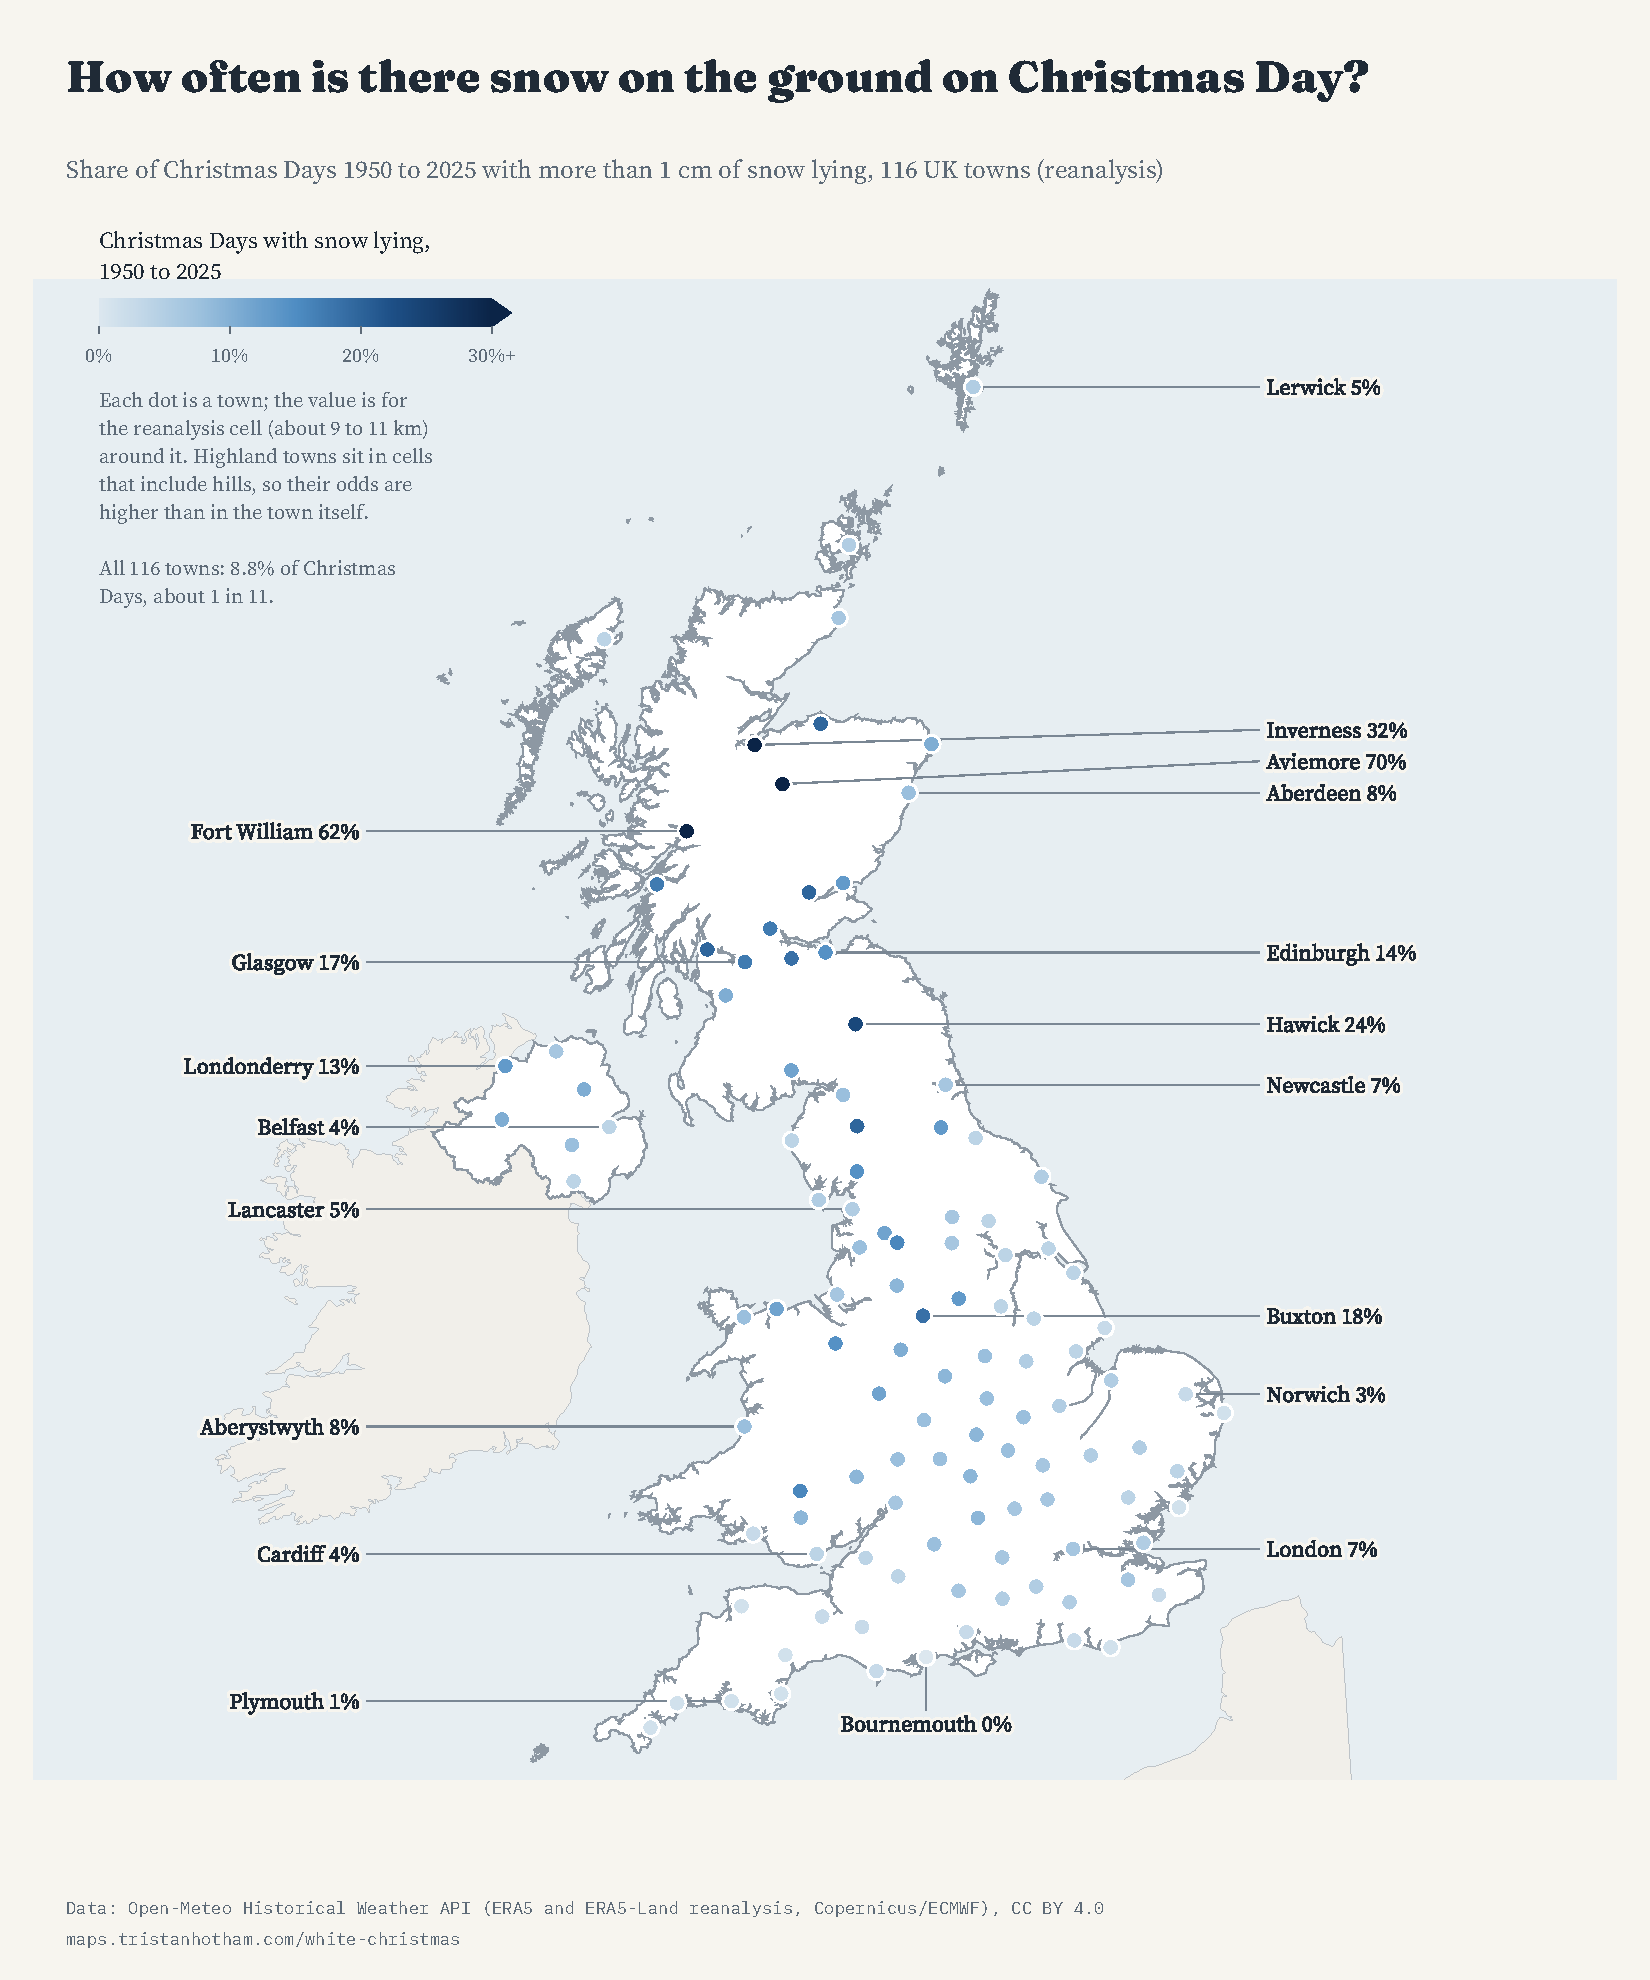
\includegraphics[width=0.86\textwidth]{f_map.pdf}
\caption{Share of Christmas Days 1950 to 2025 with more than 1 cm of snow lying in the reanalysis cell around each of the 116 towns. Labels give the share for selected towns.}\label{fig:map}
\end{figure}

\begin{table}[tbp]\centering\footnotesize\caption{Odds of a white Christmas by town: share of Christmas Days with snow lying (1950 to 2025, Wilson 95\% interval), falling (1940 to 2025) and both (1950 to 2025), and the last year with lying snow. All towns are in Appendix Table~\ref{tab:all}.}\label{tab:towns}\setlength{\tabcolsep}{4pt}\begin{tabular}{llrlrrr}\toprule Town & Nation & Height (m) & Lying \% [95\% CI] & Falling \% & Both \% & Last lying\\\midrule
\multicolumn{7}{l}{\textit{Ten highest (lying snow)}}\\
Aviemore & Scotland & 215 & 69.7 [58.7, 78.9] & 15.1 & 15.8 & 2023\\
Fort William & Scotland & 16 & 61.8 [50.6, 71.9] & 9.3 & 9.2 & 2023\\
Inverness & Scotland & 13 & 31.6 [22.2, 42.7] & 27.9 & 15.8 & 2023\\
Hawick & Scotland & 110 & 23.7 [15.5, 34.4] & 22.1 & 13.2 & 2017\\
Elgin & Scotland & 18 & 19.7 [12.3, 30.0] & 31.4 & 14.5 & 2010\\
Perth & Scotland & 13 & 19.7 [12.3, 30.0] & 25.6 & 10.5 & 2013\\
Penrith & England & 134 & 19.7 [12.3, 30.0] & 20.9 & 11.8 & 2010\\
Greenock & Scotland & 9 & 19.7 [12.3, 30.0] & 2.3 & 2.6 & 2010\\
Bathgate & Scotland & 137 & 18.4 [11.3, 28.6] & 19.8 & 9.2 & 2017\\
Buxton & England & 312 & 18.4 [11.3, 28.6] & 16.3 & 7.9 & 2010\\
\midrule\multicolumn{7}{l}{\textit{Ten lowest}}\\
Bournemouth & England & 12 & 0.0 [0.0, 4.8] & 1.2 & 0.0 & \\
Clacton & England & 15 & 1.3 [0.2, 7.1] & 2.3 & 0.0 & 1981\\
Paignton & England & 16 & 1.3 [0.2, 7.1] & 3.5 & 0.0 & 2010\\
St Austell & England & 77 & 1.3 [0.2, 7.1] & 4.7 & 0.0 & 2010\\
Falmouth & England & 43 & 1.3 [0.2, 7.1] & 4.7 & 0.0 & 2010\\
Lowestoft & England & 7 & 1.3 [0.2, 7.1] & 5.8 & 0.0 & 1981\\
Barnstaple & England & 14 & 1.3 [0.2, 7.1] & 5.8 & 0.0 & 2010\\
Plymouth & England & 15 & 1.3 [0.2, 7.1] & 7.0 & 0.0 & 2010\\
Exeter & England & 52 & 1.3 [0.2, 7.1] & 7.0 & 0.0 & 2010\\
Eastbourne & England & 12 & 1.3 [0.2, 7.1] & 7.0 & 0.0 & 1970\\
\midrule\multicolumn{7}{l}{\textit{Largest cities}}\\
Glasgow & Scotland & 38 & 17.1 [10.3, 27.1] & 19.8 & 6.6 & 2010\\
Edinburgh & Scotland & 72 & 14.5 [8.3, 24.1] & 19.8 & 7.9 & 2017\\
Manchester & England & 48 & 9.2 [4.5, 17.8] & 15.1 & 5.3 & 2010\\
Birmingham & England & 151 & 7.9 [3.7, 16.2] & 3.5 & 2.6 & 2010\\
London & England & 23 & 6.6 [2.8, 14.5] & 9.3 & 2.6 & 2010\\
Belfast & Northern Ireland & 7 & 4.0 [1.4, 11.0] & 8.1 & 2.6 & 2010\\
Cardiff & Wales & 17 & 4.0 [1.4, 11.0] & 3.5 & 2.6 & 2010\\
\bottomrule\end{tabular}\end{table}

The values for Aviemore and Fort William need a caveat that applies, more weakly, everywhere. ERA5-Land models snow depth for the average terrain of a cell about 9 to 11 km across. Aviemore's cell includes the lower slopes of the Cairngorms and averages 279 m; Fort William's includes part of the Nevis range. In an exploratory extension of M2, the odds of lying snow rise with the cell's excess height over the town (odds ratio 3.33 per 100 m, 95\% CI 1.56 to 7.12), holding the town's own height, latitude, longitude and distance to the sea constant, while the odds of falling snow do not (0.84, CI 0.52 to 1.36). This is what one would expect if lying-snow figures for towns in hilly cells partly describe the hills. Combined with the known tendency of ERA5-Land to overestimate mountain snow \citep{kouki2023,monteiro2023}, the Highland figures should be read as odds for the surrounding area, not for the town centre.

Figure~\ref{fig:strip} shows every town and every Christmas as a calendar strip. It makes the most important feature of the data visible at a glance: white Christmases come in a small number of years in which snow fell or lay across much of the country (among them 1950, 1956, 1968, 1981, 1993, 1995, 2009 and 2010), with isolated snow in the north in between.

\begin{figure}[tbp]\centering
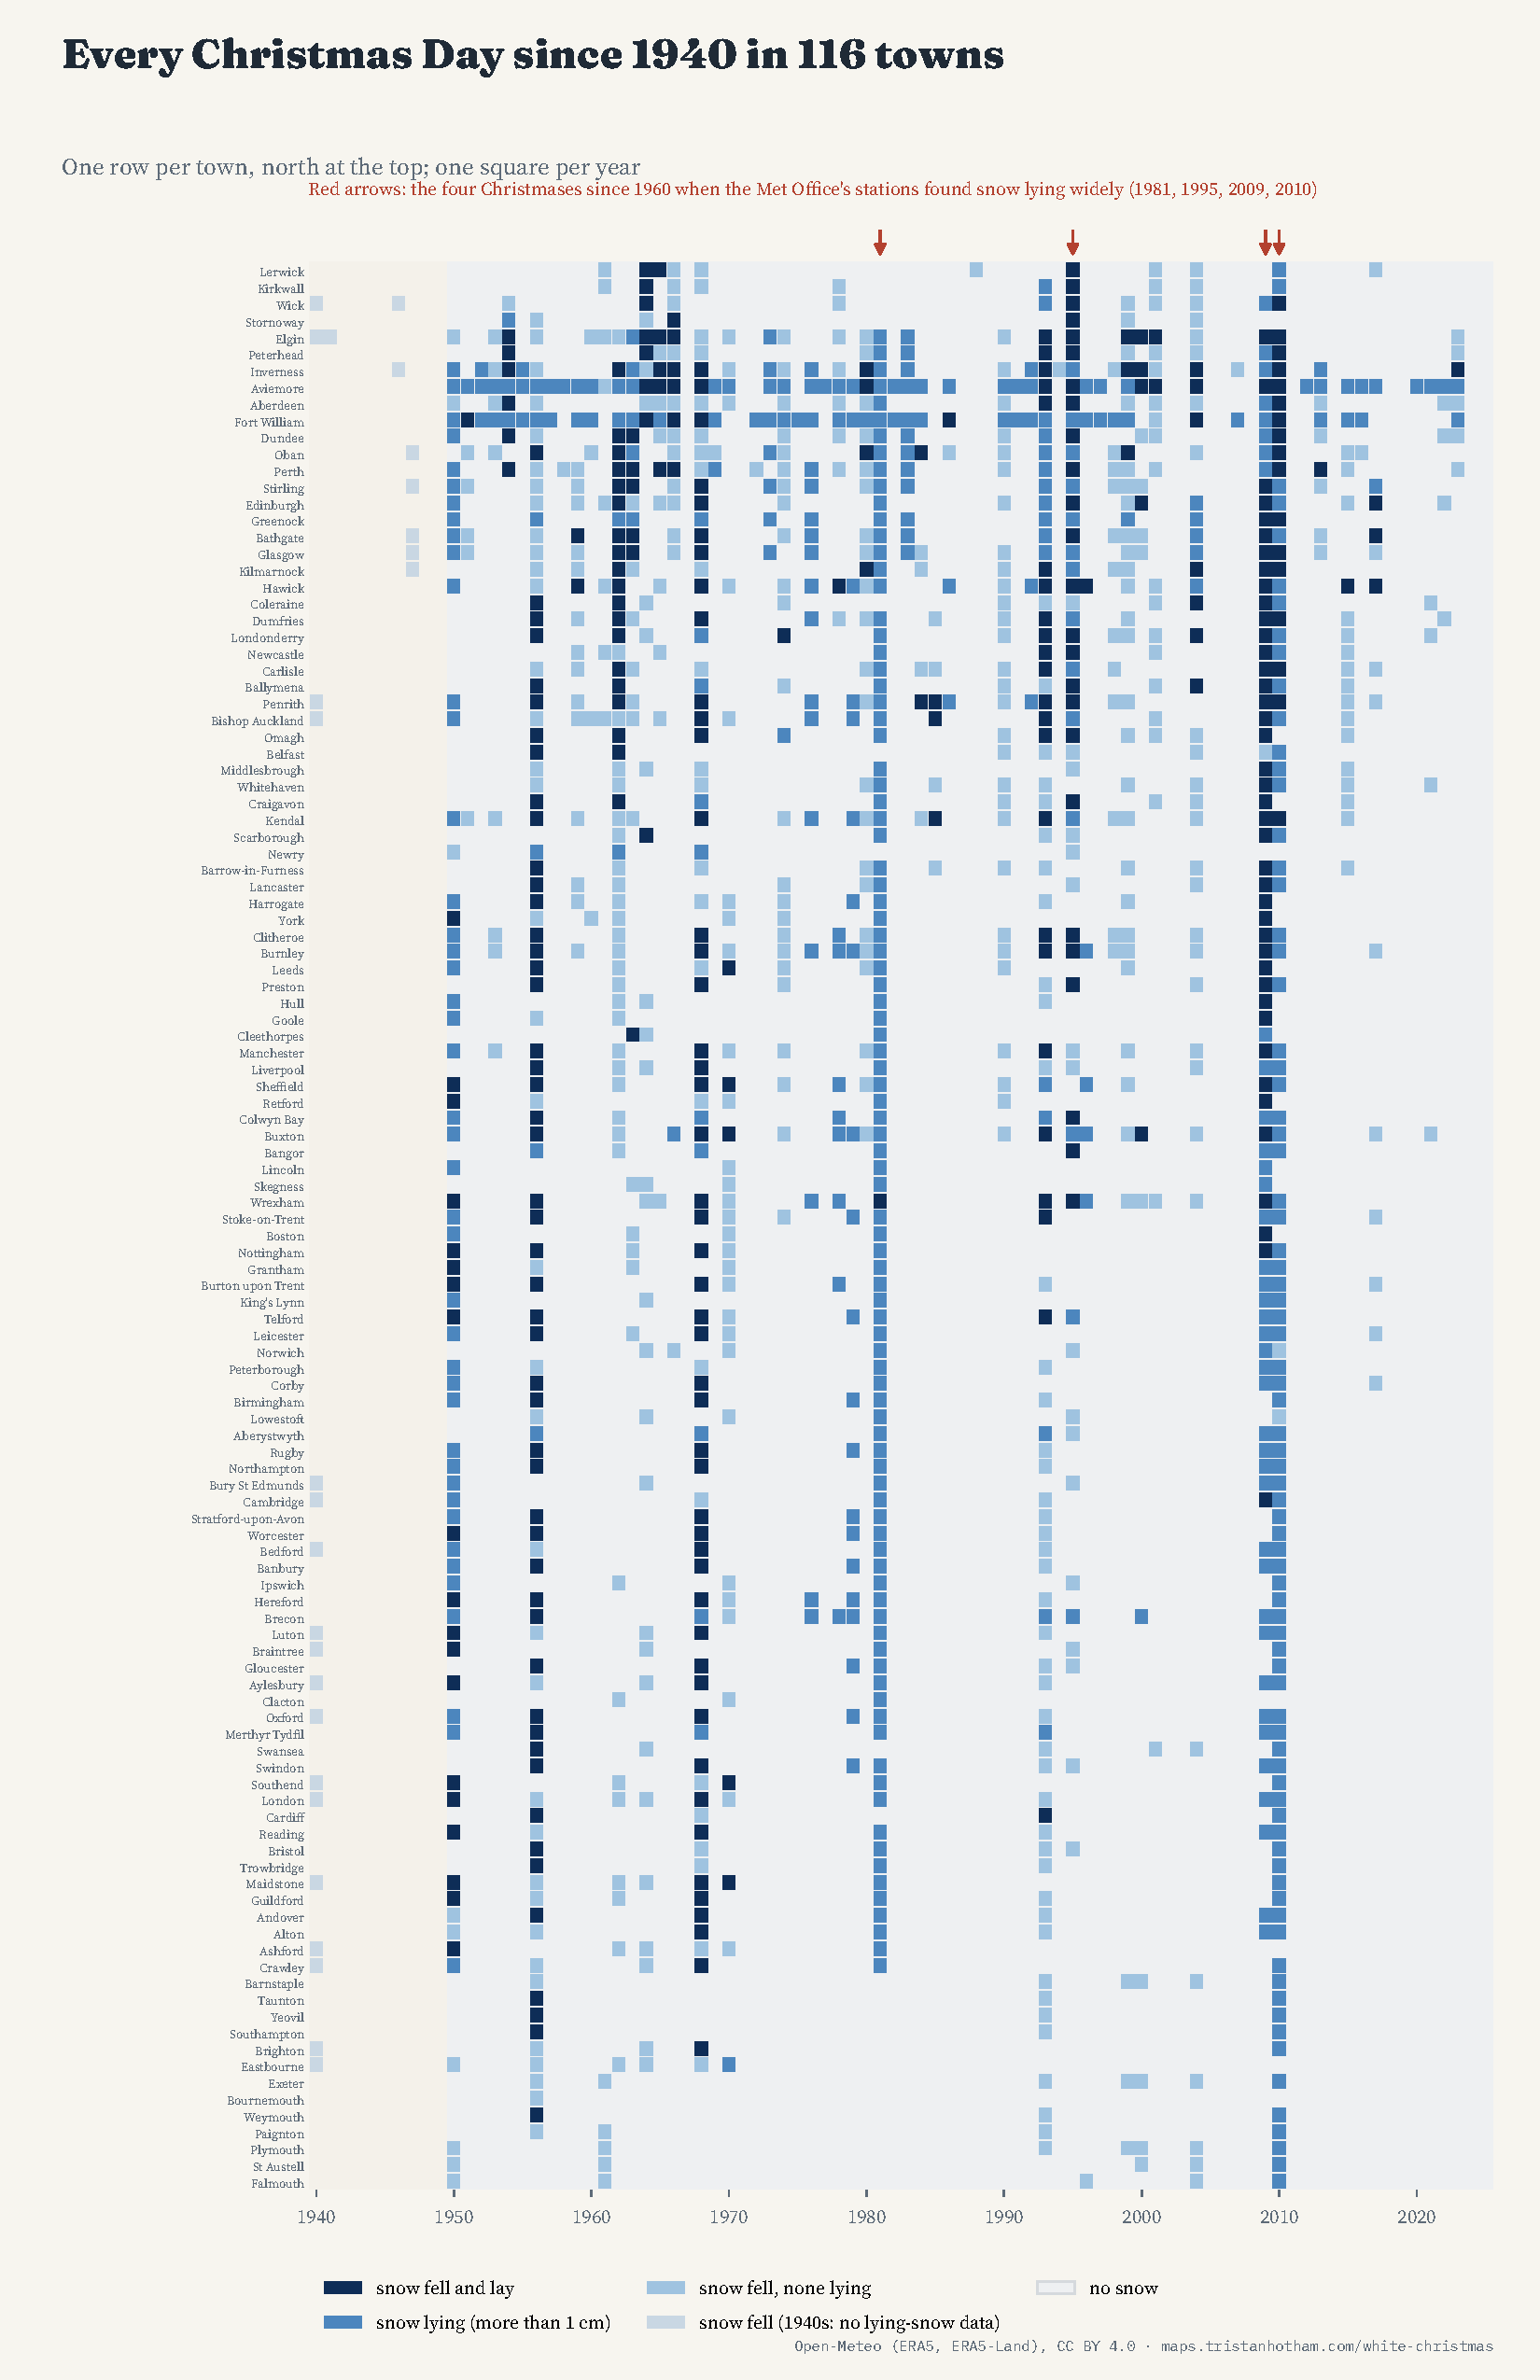
\includegraphics[width=0.93\textwidth]{f_strip.pdf}
\caption{Every Christmas Day 1940 to 2025 in the 116 towns, ordered from north to south. Lying snow is not available before 1950. Arrows mark the four widespread lying-snow Christmases since 1960 in the Met Office record.}\label{fig:strip}
\end{figure}

\subsection{Height and latitude}
Table~\ref{tab:geo} reports model M2. Holding latitude, longitude and distance to the sea constant, each 100 m of height multiplies the odds of lying snow by 3.39 (95\% CI 1.67 to 6.85) and each degree further north by 1.65 (1.29 to 2.11). For falling snow the corresponding odds ratios are 1.90 (1.29 to 2.78) and 1.39 (1.21 to 1.60). Longitude and distance to the sea have intervals that include no effect once errors are clustered by both town and year; with errors clustered by year only, towns further inland and further west had slightly higher odds of lying snow, which the two-way clustering does not confirm. Both H2 hypotheses are supported. Figure~\ref{fig:geo} shows the town-level pattern: across towns, the share of Christmases with lying snow is correlated with height (Spearman $\rho$ = 0.46) and latitude ($\rho$ = 0.59); for falling snow the correlation with latitude is strong ($\rho$ = 0.66) and with height weak ($\rho$ = 0.16).

\begin{table}[tbp]\centering\small\caption{Geography of the odds (M2): odds ratios [95\% CI] from logistic regressions with year fixed effects, standard errors clustered by town and by year. Lying and both 1950 to 2025; falling 1940 to 2025.}\label{tab:geo}\begin{tabular}{llll}\toprule & Lying & Falling & Both\\\midrule
Height (per 100 m) & 3.39 [1.67, 6.85] & 1.90 [1.29, 2.78] & 1.92 [1.36, 2.71]\\
Latitude (per degree N) & 1.65 [1.29, 2.11] & 1.39 [1.21, 1.60] & 1.45 [1.18, 1.79]\\
Longitude (per degree E) & 0.81 [0.65, 1.02] & 0.94 [0.83, 1.07] & 0.86 [0.73, 1.02]\\
Distance to the sea (per 10 km) & 1.14 [1.00, 1.30] & 0.91 [0.80, 1.04] & 1.11 [0.96, 1.29]\\
\midrule Town-years used & 6,728 & 5,800 & 3,712\\
Years dropped (no town with the outcome) & 18 & 36 & 44\\
\midrule\multicolumn{4}{l}{\textit{Exploratory (added after the plan): with the ERA5-Land cell's height}}\\
Height (per 100 m) & 3.25 [1.69, 6.23] & 1.91 [1.31, 2.80] & \\
Cell height above the town (per 100 m) & 3.33 [1.56, 7.12] & 0.84 [0.52, 1.36] & \\
\bottomrule\end{tabular}\end{table}

\begin{figure}[tbp]\centering
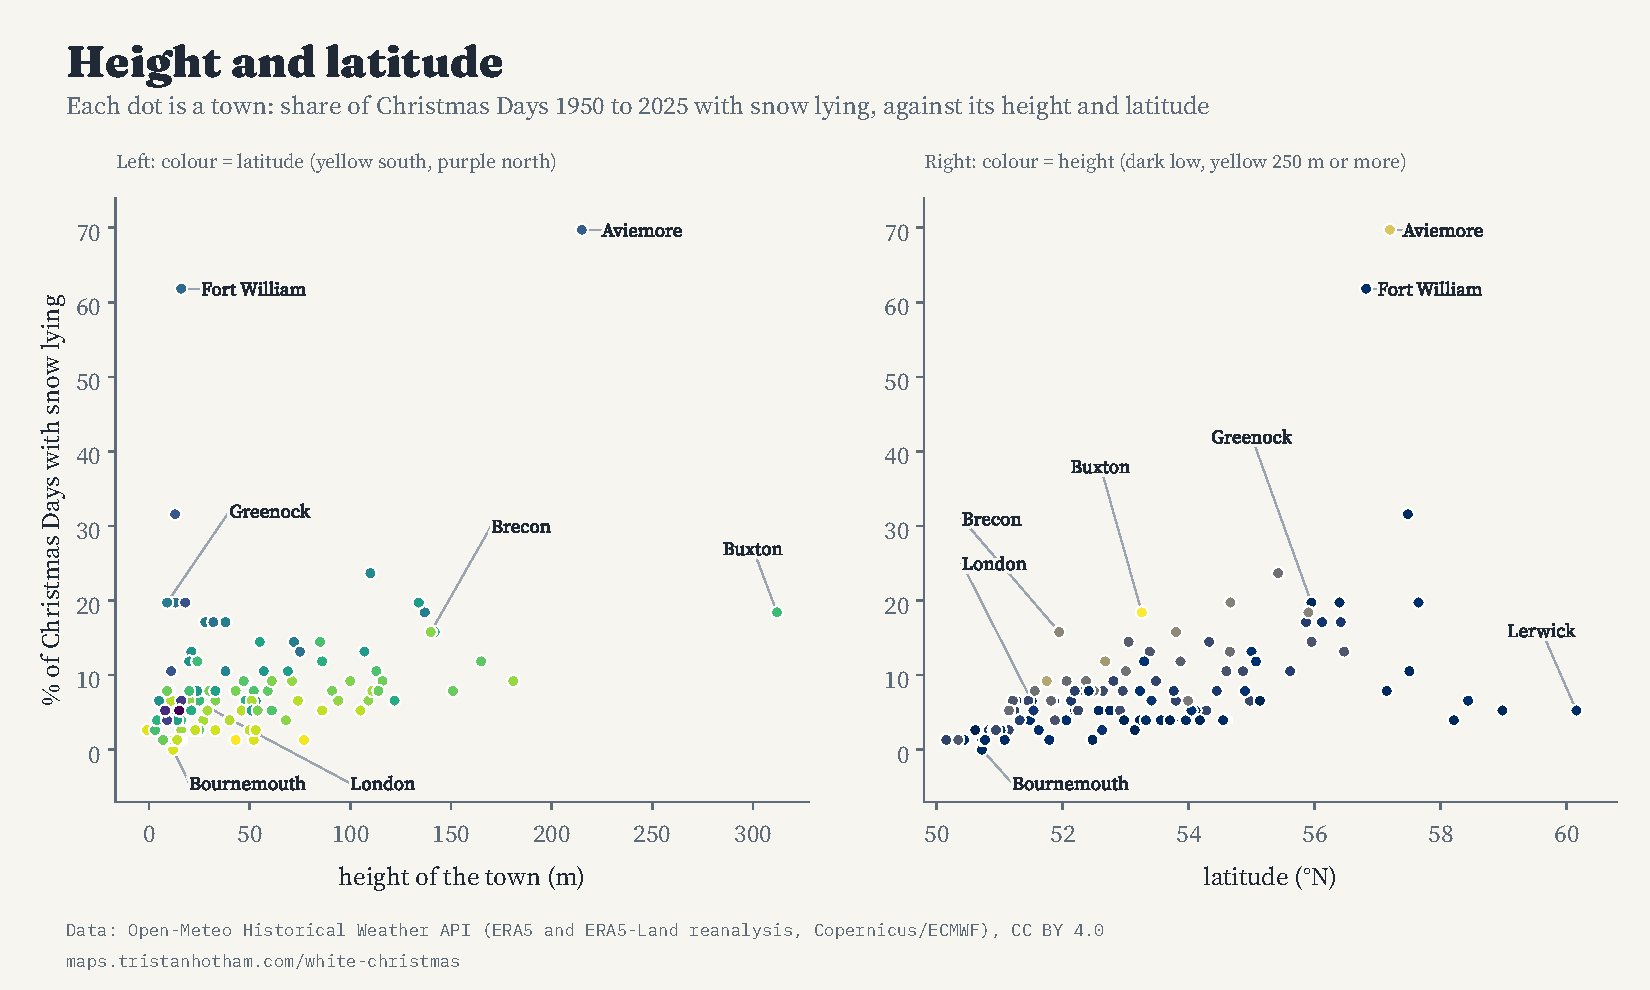
\includegraphics[width=\textwidth]{f_geo.pdf}
\caption{Share of Christmas Days with lying snow by town, against the town's height (left, coloured by latitude) and latitude (right, coloured by height).}\label{fig:geo}
\end{figure}

\subsection{Does the reanalysis match the station record?}
The validation is the strongest result in the paper. Ranking the 66 Christmases from 1960 to 2025 by the share of towns with lying snow, the Met Office's four widespread years come first (2010, 83\% of towns), second (1981, 81\%), third (2009, 69\%) and fifth (1995, 34\%). The probability that four years chosen at random would all rank fifth or higher is about 7 in a million. The reanalysis also agrees on the detail of 1981, when snow that had fallen earlier lay widely but little fell on the day: 81\% of towns had lying snow but only 1 of the 116 had falling snow. Figure~\ref{fig:valid} compares the town shares with the published station shares: for falling snow the rank correlation across eight years is 0.93, and for lying snow across six years 0.65, with 2010 matching closely (83\% of stations, 83\% of towns), 2009 somewhat higher in the towns (69\% against 57\%) and 2020 to 2023 near zero in both. The reanalysis shows more falling snow than the stations in 2009 (36\% of towns against 13\% of stations), consistent with a grid-cell average spreading light snow more widely than single sites record. By V3, falling snow reached 5\% or more of towns in 27 of 66 years since 1960 (41\%), somewhat below the Met Office's ``around half'' of years for its stations, which is the expected direction for a measure that cannot see isolated flakes.

\begin{figure}[tbp]\centering
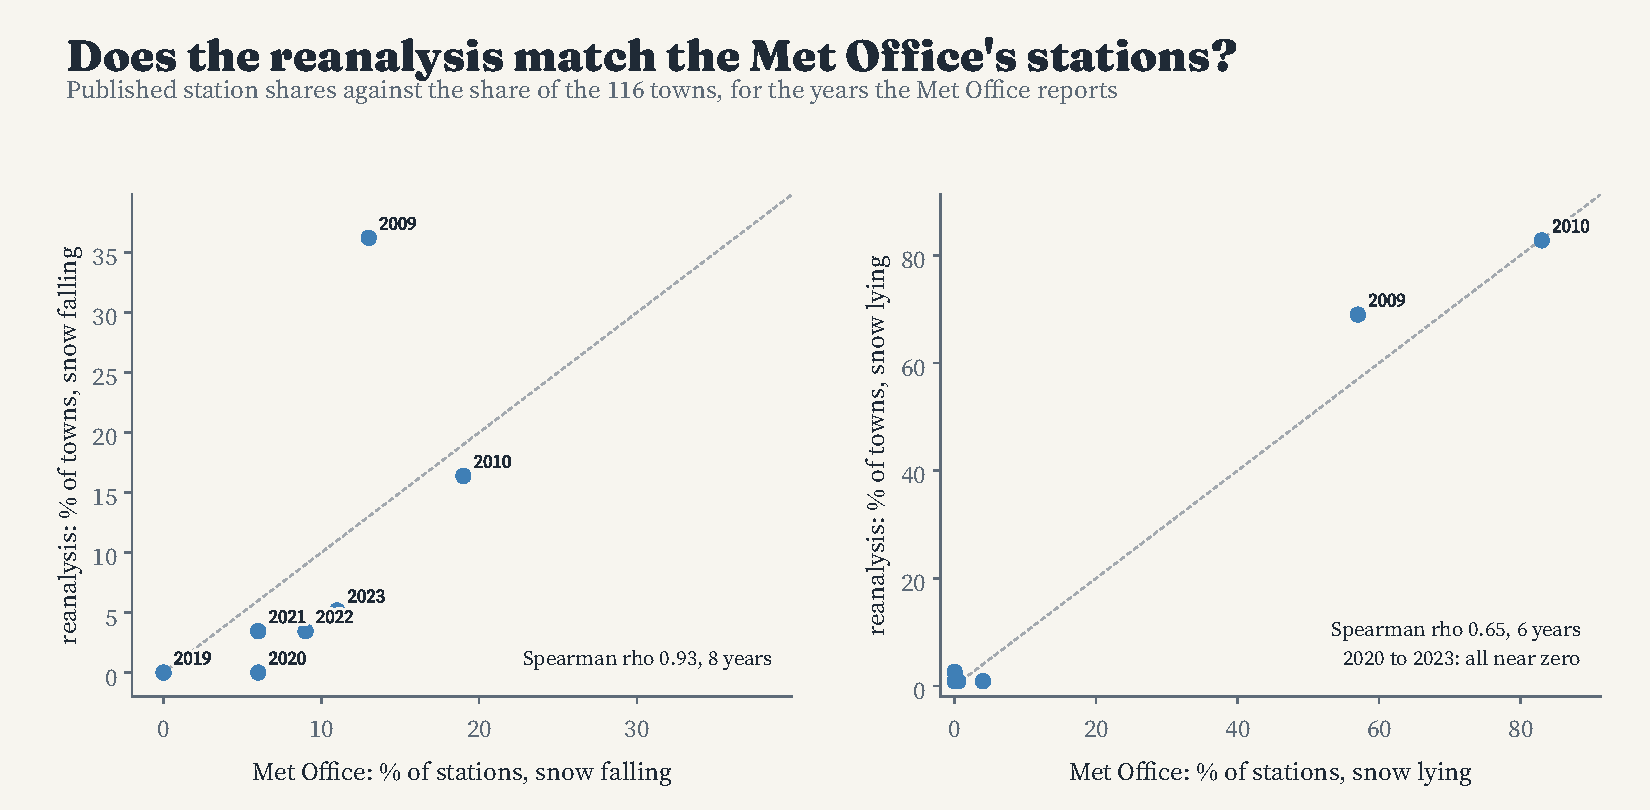
\includegraphics[width=\textwidth]{f_valid.pdf}
\caption{Validation: Met Office station shares on Christmas Day (where published) against the share of the 116 towns in the reanalysis, for falling (left) and lying (right) snow. The dotted line marks equality.}\label{fig:valid}
\end{figure}

\begin{table}[tbp]\centering\small\caption{Validation against the Met Office's published Christmas Day figures: percentage of stations and of the 116 towns with snow lying and falling. Widespread lying-snow years since 1960 (1981, 1995, 2009, 2010) rank 2, 5, 3, 1 of 66 by the share of towns. Spearman $\rho$: lying 0.65 (6 years), falling 0.93 (8 years).}\label{tab:valid}\begin{tabular}{lrrrr}\toprule & \multicolumn{2}{c}{Lying} & \multicolumn{2}{c}{Falling}\\\cmidrule(lr){2-3}\cmidrule(lr){4-5} Year & Stations \% & Towns \% & Stations \% & Towns \%\\\midrule
2009 & 57 & 69.0 & 13 & 36.2\\
2010 & 83 & 82.8 & 19 & 16.4\\
2018 &  &  & 0 & 0.0\\
2019 &  &  & 0 & 0.0\\
2020 & 4 & 0.9 & 6 & 0.0\\
2021 & $<$1 & 0.9 & 6 & 3.4\\
2022 & 0 & 0.9 & 9 & 3.4\\
2023 & 0 & 2.6 & 11 & 5.2\\
\bottomrule\end{tabular}\end{table}

\subsection{Has a white Christmas become rarer?}
Table~\ref{tab:trend} reports the planned trend tests and Figures~\ref{fig:annual} and~\ref{fig:decade} show the series. By decade, lying snow was found on 12.4\% of town Christmases in the 1950s, 10.3\% in the 1960s, between 6.1\% and 10.7\% from the 1970s to the 2010s, and 0.9\% in the six Christmases from 2020 to 2025. Falling snow is more erratic: 19.1\% in the 1960s, 3.7\% in the 1980s, 15.9\% in the 1990s and 2.0\% in the 2020s. Splitting 1950 to 2025 into two halves of 38 years, lying snow fell from 10.4\% of town Christmases (1950 to 1987) to 7.3\% (1988 to 2025), and falling snow from 11.0\% to 8.3\%.

The planned main model does not detect a decline that can be told apart from chance. For lying snow, the odds ratio per decade is 0.89 (95\% CI 0.68 to 1.16, $p$ = 0.39), implying a probability at the average town of 12.4\% in 1950 and 6.0\% in 2025, but with an interval wide enough to include no change. For falling snow from 1940 the odds ratio is 0.94 (0.82 to 1.08), and for both together from 1950 0.82 (0.62 to 1.09). By the plan's own criterion, these count against H1.

The second planned test points the other way for lying snow. The Mann-Kendall test on the national annual share finds a significant decline (Kendall's $\tau$ = $-$0.23, $p$ = 0.004; Sen's slope $-$0.36 percentage points of towns a decade). The two tests disagree because they weigh the data differently. The logistic model is dominated by the few Christmases with snow almost everywhere, and two of the largest, 2009 and 2010, are recent. The rank test counts how often one year is snowier than another, and recent decades have many more Christmases with no lying snow in any town: 4 of 38 Christmases from 1950 to 1987 against 14 of 38 from 1988 to 2025. Christmases with lying snow in at least 10\% of towns went from 9 to 5, and none since 2010. For falling snow and for both together the rank tests are not significant ($p$ = 0.56 and 0.08).

The mechanism is visible in temperature. Christmas Day maximum temperature, averaged across towns, rose by 0.49\,°C a decade from 1950 (95\% CI 0.17 to 0.81), about 0.5\,°C a decade by Sen's slope. From 1940 the rise is smaller and not significant (0.25\,°C a decade, CI $-$0.03 to 0.52), because the Christmases of the 1940s were mild in the reanalysis (a mean maximum of 7.2\,°C, against 3.0\,°C in the 1970s and 8.0\,°C in the 2010s).

\begin{table}[tbp]\centering\small\caption{Trend tests. M1: odds ratio per decade [95\% CI] from logistic regression with town fixed effects, standard errors clustered by year (towns with no variation drop out). M1b: Mann-Kendall test on the annual share of towns.}\label{tab:trend}\begin{tabular}{p{4.4cm}lrrrr}\toprule & \multicolumn{3}{c}{M1} & \multicolumn{2}{c}{M1b}\\\cmidrule(lr){2-4}\cmidrule(lr){5-6} Outcome & OR per decade & $p$ & Town-years / years & $\tau$ & $p$\\\midrule
Lying (1950 to 2025) & 0.89 [0.68, 1.16] & 0.386 & 8,740 / 76 & $-$0.23 & 0.004\\
Falling (1940 to 2025) & 0.94 [0.82, 1.08] & 0.375 & 9,976 / 86 & $-$0.05 & 0.555\\
Falling (1950 to 2025) & 0.83 [0.69, 1.00] & 0.052 & 8,816 / 76 & $-$0.14 & 0.083\\
Both (1950 to 2025) & 0.82 [0.62, 1.09] & 0.172 & 7,372 / 76 & $-$0.15 & 0.079\\
\midrule Christmas Day max. temperature, 1950 to 2025 (°C a decade, OLS) & 0.49 [0.17, 0.81] & 0.002 & 8,816 / 76 & 0.21 & 0.008\\
Christmas Day max. temperature, 1940 to 2025 & 0.25 [$-$0.03, 0.52] & 0.077 & 9,976 / 86 & 0.12 & 0.103\\
\bottomrule\end{tabular}\end{table}

\begin{figure}[tbp]\centering
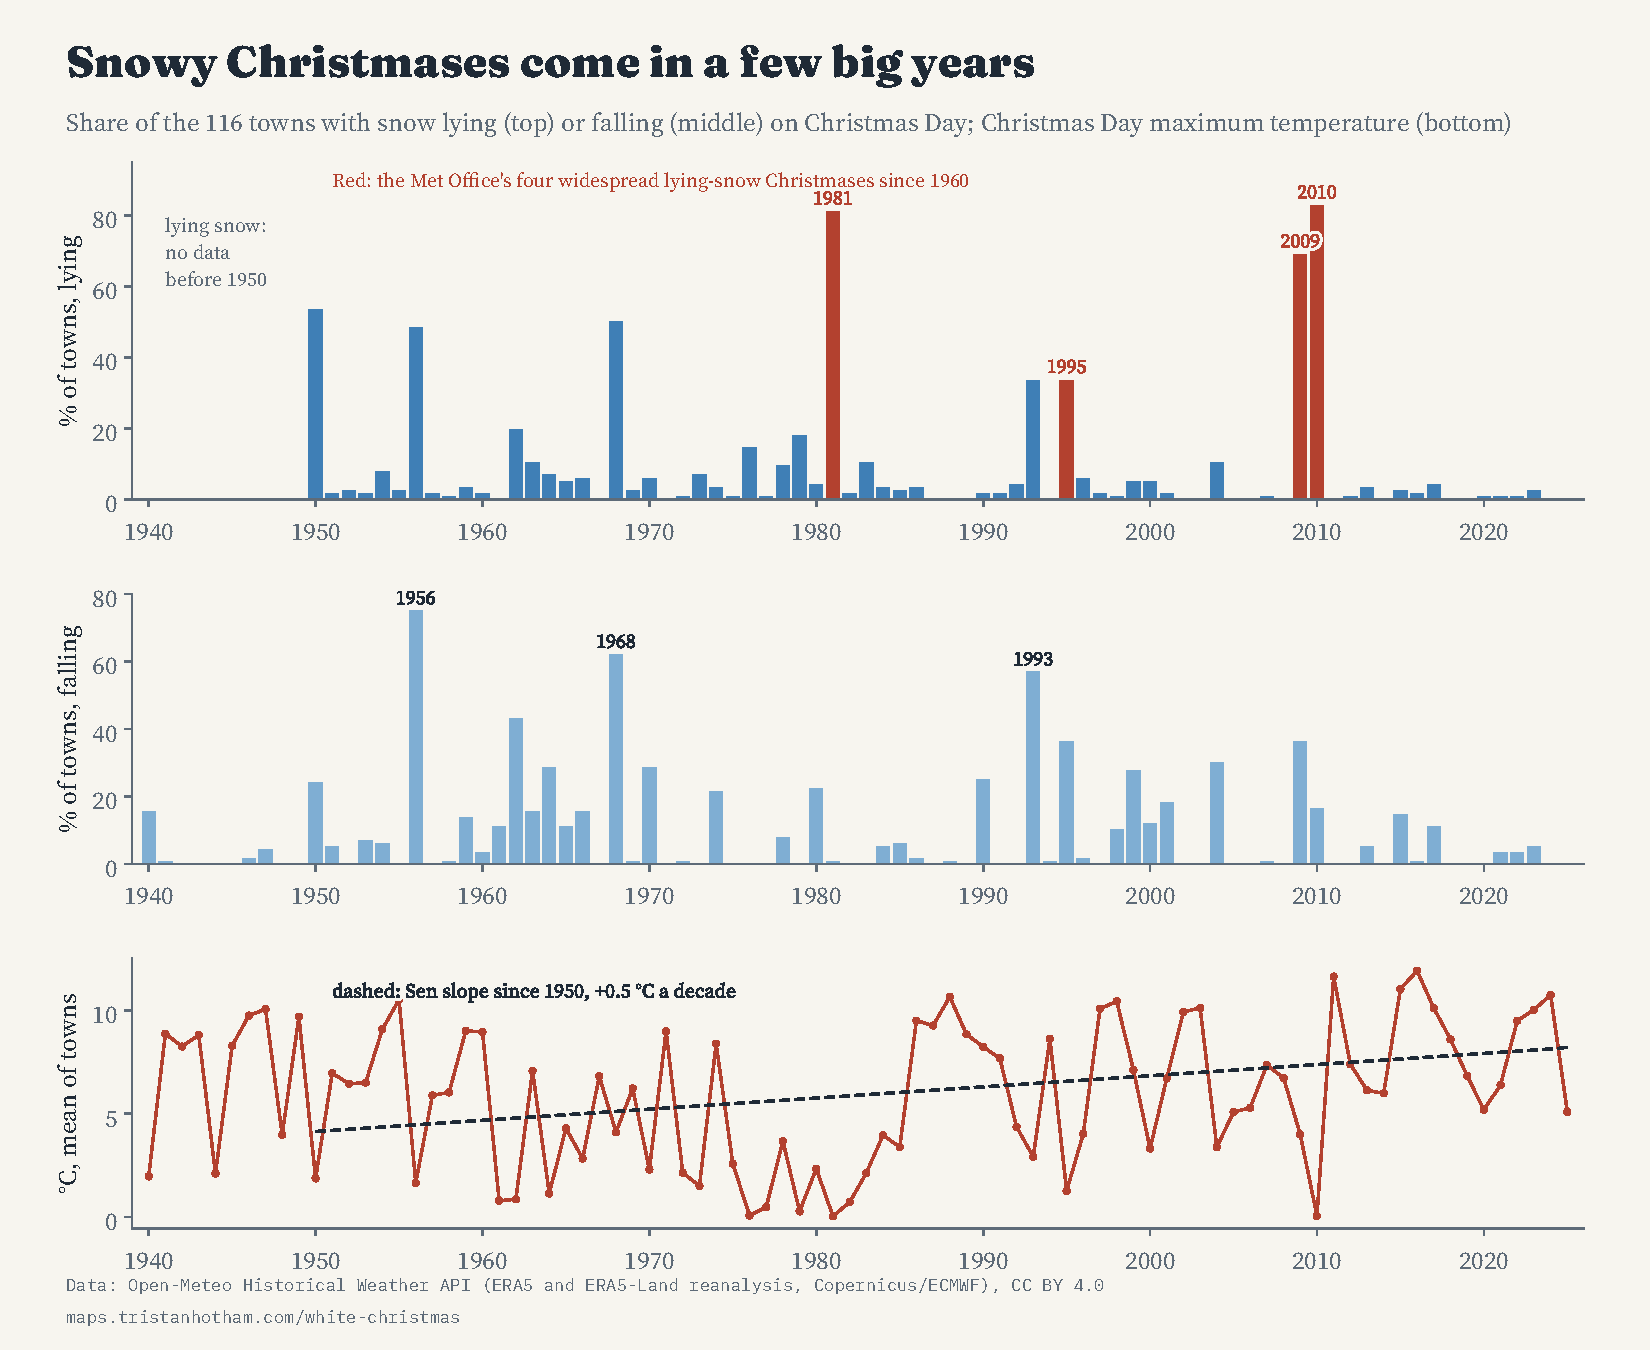
\includegraphics[width=\textwidth]{f_annual.pdf}
\caption{Share of the 116 towns with snow lying (top, from 1950) and falling (middle) on Christmas Day, and the mean Christmas Day maximum temperature (bottom) with Sen's slope since 1950. Red bars: the Met Office's four widespread lying-snow Christmases since 1960.}\label{fig:annual}
\end{figure}

\begin{figure}[tbp]\centering
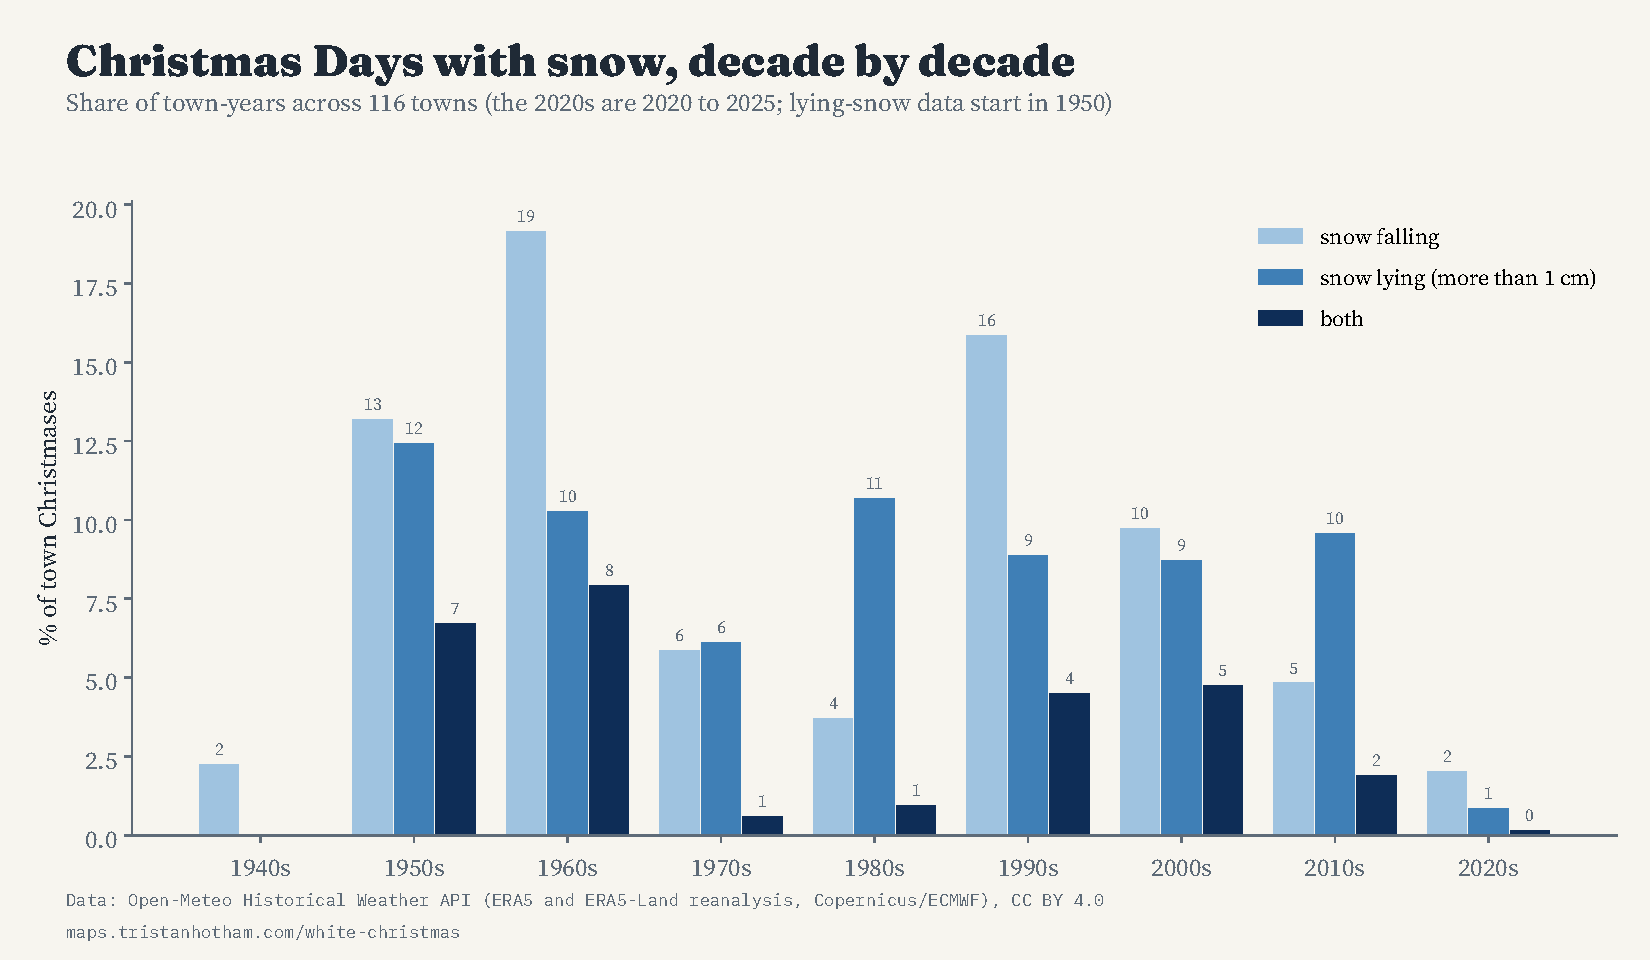
\includegraphics[width=\textwidth]{f_decade.pdf}
\caption{Share of town Christmases with snow falling, lying and both, by decade. The 1940s have no lying-snow data and the 2020s cover six years.}\label{fig:decade}
\end{figure}

\section{Robustness}\label{sec:robust}
Table~\ref{tab:robust} and Figure~\ref{fig:robust} report every planned check. For lying snow, all 11 checks give odds ratios below 1, from 0.72 to 0.98, but only one excludes 1: leaving out 2009 and 2010, which gives 0.72 per decade (0.57 to 0.89, $p$ = 0.003). Ending in 2016 moves the estimate towards no change (0.98), because the last nine Christmases are among the least snowy; this check targets a possible break in snowfall and temperature, not in snow depth. The linear probability model gives $-$0.84 percentage points a decade ($-$2.64 to 0.95). For falling snow, 9 of 11 checks are below 1 and one excludes it: starting in 1960 (0.80, 0.65 to 0.99). Starting in 1950 gives 0.83 (0.69 to 1.00). The falling-snow trend therefore depends on the start year, and in particular on the 1940s, when the reanalysis shows snow falling on only 2.2\% of town Christmases, far fewer than in the 1950s (13.2\%). That may be real (those Christmases were mild in the same data, with a mean maximum of 7.2\,°C) or may reflect the thinner observations constraining ERA5 before 1950 \citep{bell2021}; I cannot tell which.

The permutation test (P1) places the observed slope for lying snow at the 0.18 quantile of 2,000 slopes from shuffled years (two-sided $p$ = 0.36), and for falling snow at 0.25 ($p$ = 0.48), agreeing with the clustered model. In the persistence placebo (P2), snow lying on 24 December was still lying on the 25th in 86\% of 732 cases, with no trend in the logistic model (0.97 per decade, 0.71 to 1.33). The rank test on the annual share of persisting snow is significant ($p$ = 0.03), but that series exists only in the 58 years with any snow on the 24th and is mostly 0 or 100\%, so I do not read it as evidence of drift.

\begin{figure}[tbp]\centering
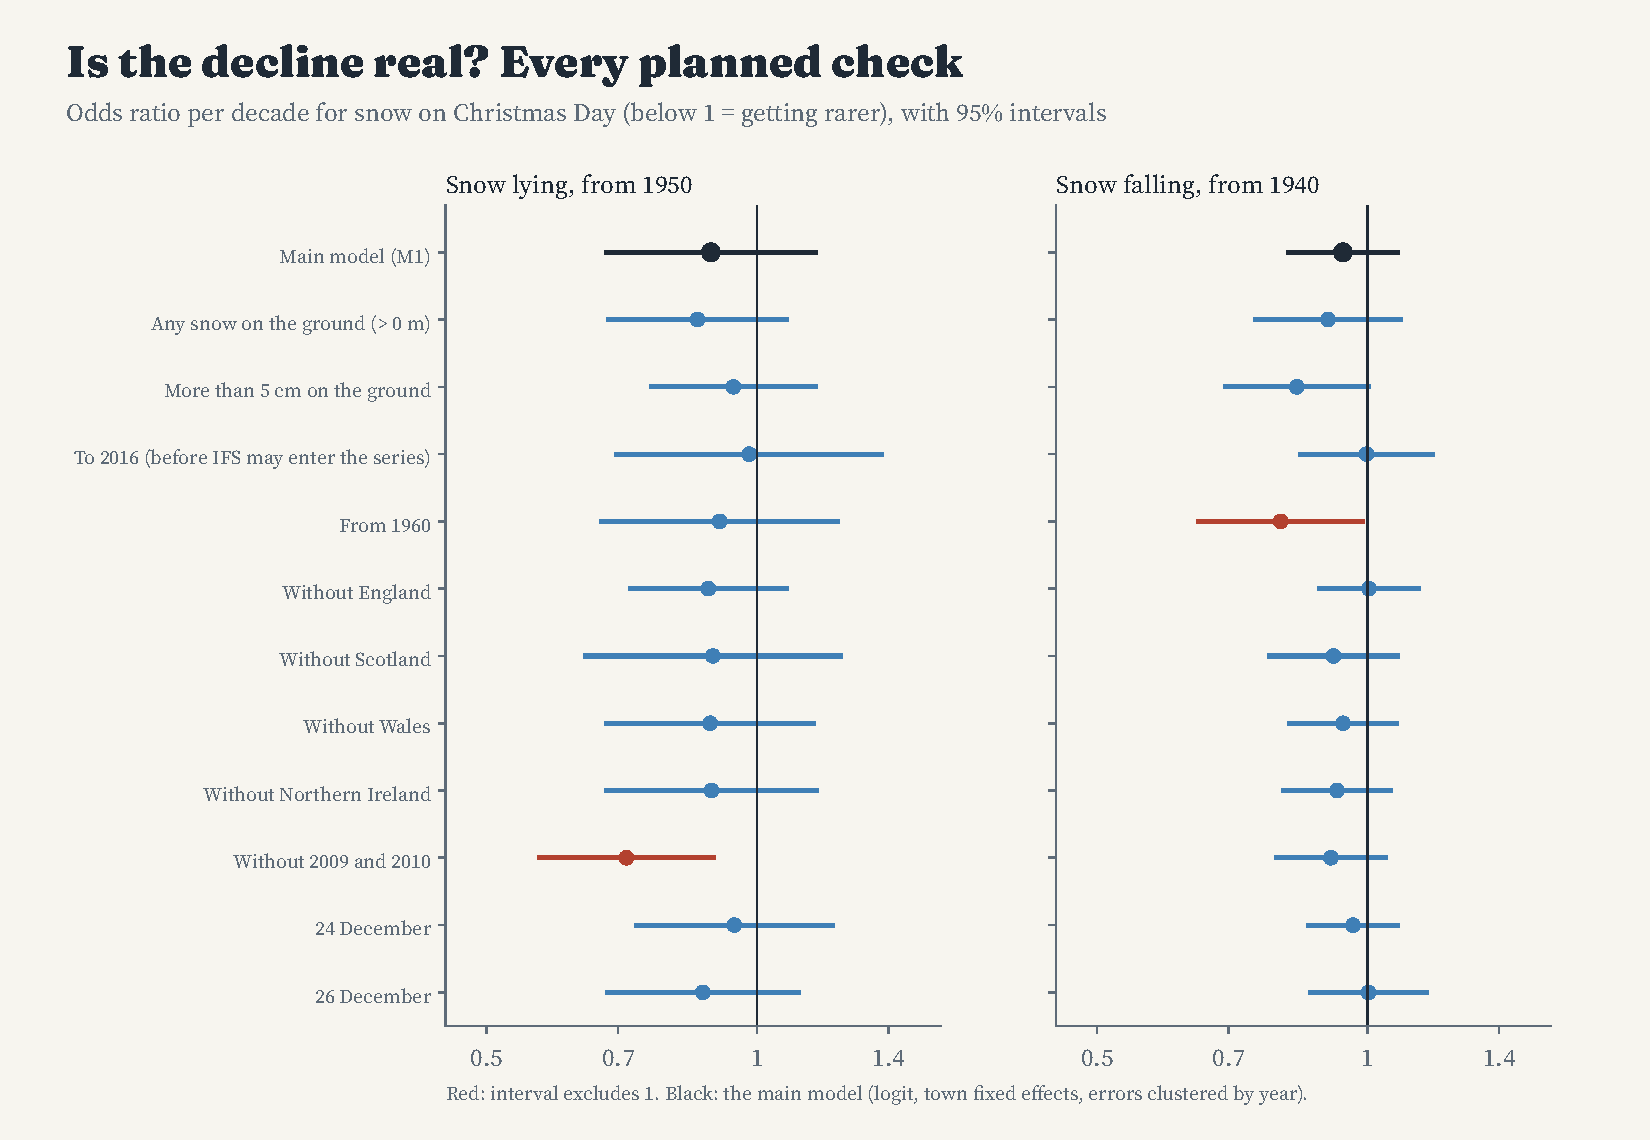
\includegraphics[width=\textwidth]{f_robust.pdf}
\caption{Every planned check of the trend: odds ratio per decade with 95\% confidence interval for lying (left) and falling (right) snow. Red: interval excludes 1.}\label{fig:robust}
\end{figure}

\begin{table}[tbp]\centering\small\caption{Robustness and falsification: odds ratio per decade [95\% CI], $p$, and town-years / years used.}\label{tab:robust}\begin{tabular}{p{7.6cm}lrr}\toprule Check & Estimate & $p$ & N\\\midrule
\multicolumn{4}{l}{\textit{Lying snow, from 1950}}\\
\quad Main model (M1) & 0.89 [0.68, 1.16] & 0.386 & 8,816 / 76\\
\quad Any snow on the ground (> 0 m) & 0.86 [0.68, 1.08] & 0.189 & 8,816 / 76\\
\quad More than 5 cm on the ground & 0.94 [0.76, 1.16] & 0.570 & 8,816 / 76\\
\quad To 2016 (before IFS may enter the series) & 0.98 [0.70, 1.38] & 0.907 & 7,772 / 67\\
\quad From 1960 & 0.91 [0.67, 1.23] & 0.534 & 7,656 / 66\\
\quad Without England & 0.88 [0.72, 1.08] & 0.218 & 2,736 / 76\\
\quad Without Scotland & 0.89 [0.64, 1.24] & 0.497 & 7,220 / 76\\
\quad Without Wales & 0.89 [0.68, 1.16] & 0.374 & 8,208 / 76\\
\quad Without Northern Ireland & 0.89 [0.68, 1.17] & 0.396 & 8,284 / 76\\
\quad Without 2009 and 2010 & 0.72 [0.57, 0.89] & 0.003 & 8,584 / 74\\
\quad 24 December & 0.94 [0.73, 1.21] & 0.648 & 8,816 / 76\\
\quad 26 December & 0.87 [0.68, 1.11] & 0.264 & 8,816 / 76\\
\multicolumn{4}{l}{\textit{Falling snow, from 1940}}\\
\quad Main model (M1) & 0.94 [0.82, 1.08] & 0.375 & 9,976 / 86\\
\quad At least 0.7 cm of snowfall (1 mm water) & 0.90 [0.75, 1.09] & 0.285 & 9,976 / 86\\
\quad From 1950 & 0.83 [0.69, 1.00] & 0.052 & 8,816 / 76\\
\quad To 2016 (before IFS may enter the series) & 1.00 [0.84, 1.18] & 0.974 & 8,932 / 77\\
\quad From 1960 & 0.80 [0.65, 0.99] & 0.038 & 7,656 / 66\\
\quad Without England & 1.00 [0.88, 1.14] & 0.959 & 3,096 / 86\\
\quad Without Scotland & 0.92 [0.78, 1.08] & 0.300 & 8,170 / 86\\
\quad Without Wales & 0.94 [0.82, 1.08] & 0.372 & 9,288 / 86\\
\quad Without Northern Ireland & 0.92 [0.81, 1.06] & 0.263 & 9,374 / 86\\
\quad Without 2009 and 2010 & 0.91 [0.79, 1.05] & 0.187 & 9,744 / 84\\
\quad 24 December & 0.96 [0.86, 1.08] & 0.516 & 9,976 / 86\\
\quad 26 December & 1.00 [0.86, 1.16] & 0.977 & 9,976 / 86\\
\midrule Linear probability model, lying (points a decade) & $-$0.84 [$-$2.64, 0.95] & 0.358 & 8,816\\
Linear probability model, falling & $-$0.48 [$-$1.57, 0.61] & 0.391 & 9,976\\
P1 permutation, lying (two-sided $p$, 2,000 shuffles) & & 0.357 & \\
P1 permutation, falling & & 0.485 & \\
P2 persistence: still lying on 25th given lying on 24th & 0.97 [0.71, 1.33] & 0.851 & 732 / 58\\
\bottomrule\end{tabular}\end{table}

\section{Discussion}\label{sec:disc}
\subsection{What the pattern says}
Three things are clear. First, a white Christmas in the sense most people imagine, snow on the ground, is uncommon almost everywhere in the United Kingdom outside the Scottish Highlands: about one Christmas in 11 across these towns, about one in 15 in London, and never in Bournemouth since 1950. Second, the odds are strongly local, rising with height and latitude in line with what is known about British snow \citep{kay2016,brown2019}. Third, white Christmases are clustered in years: most of the snowy town-years come from a handful of Christmases when snow lay across much of the country, and it is the timing of those few years that drives any trend estimate.

On the trend, the honest summary is that the evidence leans towards fewer white Christmases but does not settle it. The planned logistic model cannot rule out no change, while the planned rank test finds a decline, driven by the growing number of Christmases with no lying snow anywhere. Christmas Day has warmed significantly since 1950, consistent with the temperature sensitivity of British snow \citep{brown2019,brown2020}. But 2009 and 2010, two of the three most widespread lying-snow Christmases in 66 years, are recent, and with them in the data the decline is not statistically clear. That is exactly the pattern one would expect from a warming signal superimposed on large year-to-year variability driven by the circulation \citep{brown2020}: rarer snowy Christmases, but not impossible ones.

\subsection{Limitations}
The reanalysis is not an observation. Snowfall is a grid-cell average from a model forecast and cannot represent a single flake at a single site, which is the Met Office's betting definition; the measure of falling snow here is closer to ``measurable snow somewhere in the cell''. Snow depth comes from ERA5-Land, which is known to overestimate snow in the mountains \citep{kouki2023,monteiro2023}, and represents the cell's average terrain, so towns in hilly cells are assigned some of their hills' snow. ERA5 before 1950, and to a lesser extent the 1950s, is less constrained by observations \citep{bell2021}, and reanalyses can produce spurious long-term trends when the observing system changes \citep{monteiro2023}. From 2017 the snowfall and temperature series may come from IFS analyses rather than ERA5; the trend estimates ending in 2016 are not materially different in sign. The towns are a purposive sample, so averages across them are not averages over the population or the land. Christmas Day is one day, and the effective sample for any trend is 76 or 86 years, too few to estimate a modest trend precisely against this much variability. Finally, the validation uses only the handful of year-by-year figures the Met Office has published; a full station series would allow a stronger test.

\subsection{Implications}
For anyone who wants to know their own odds, the reanalysis gives a consistent answer for 86 Christmases that agrees well with the station record in the years that can be checked, with the clear exception that values for towns in mountainous cells describe the surrounding hills. For forecasting and betting, the distinction between snow falling and snow lying matters: falling snow on Christmas Day happens somewhere in most decades of this record, but lying snow across much of the country has happened only a few times a generation, and not since 2010. For climate communication, a single day is a poor indicator of change: the decline is plausible and consistent with warming, but its statistical clarity hinges on a few memorable Christmases.

\section{Conclusion}\label{sec:conc}
Across 116 UK towns and 86 Christmases, reanalysis data put the odds of snow lying on Christmas Day at about one in 11, from never on the south coast to most years in the Highlands, with height and latitude doing most of the work. The reanalysis reproduces the Met Office's record of widespread white Christmases almost exactly. Christmas Day has warmed and snowy Christmases have probably become rarer, but the evidence for the decline depends on how a few exceptional years are treated. The odds of a white Christmas are local, low, and decided by a handful of years.

\section*{Data availability statement}
Data and code: Zenodo DOI https://doi.org/10.5281/zenodo.24132735. The repository \url{https://github.com/Tristan-Hotham/white-christmas} holds the town-year data, every model estimate and the code from the Open-Meteo extract to every figure and number. The interactive map is at \url{https://maps.tristanhotham.com/white-christmas/}. Reanalysis data: Open-Meteo Historical Weather API, CC BY 4.0, containing modified Copernicus Climate Change Service information (ERA5, ERA5-Land).

\section*{AI statement}
I wrote the text, with drafting and editing assistance from Claude (Anthropic), which also helped prepare the analysis code. I reviewed and checked all text and results.

\begin{thebibliography}{99}
\bibitem[Bell et al.(2021)]{bell2021} Bell, B., Hersbach, H., Simmons, A., Berrisford, P., Dahlgren, P., Horányi, A., Muñoz-Sabater, J., Nicolas, J., Radu, R., Schepers, D., Soci, C., Villaume, S., Bidlot, J., Haimberger, L., Woollen, J., Buontempo, C. and Thépaut, J.-N. (2021) The ERA5 global reanalysis: preliminary extension to 1950. \textit{Quarterly Journal of the Royal Meteorological Society} 147(741), 4186 to 4227. doi:10.1002/qj.4174.
\bibitem[Brown(2019)]{brown2019} Brown, I. (2019) Snow cover duration and extent for Great Britain in a changing climate: altitudinal variations and synoptic-scale influences. \textit{International Journal of Climatology} 39(12), 4611 to 4626. doi:10.1002/joc.6090.
\bibitem[Brown(2020)]{brown2020} Brown, I. (2020) Snow cover variability in Great Britain during a changing climate. \textit{Weather} 75(2), 61 to 66. doi:10.1002/wea.3625.
\bibitem[Brown and Robinson(2011)]{brown2011} Brown, R. D. and Robinson, D. A. (2011) Northern Hemisphere spring snow cover variability and change over 1922 to 2010 including an assessment of uncertainty. \textit{The Cryosphere} 5, 219 to 229. doi:10.5194/tc-5-219-2011.
\bibitem[Cameron et al.(2011)]{cameron2011} Cameron, A. C., Gelbach, J. B. and Miller, D. L. (2011) Robust inference with multiway clustering. \textit{Journal of Business and Economic Statistics} 29(2), 238 to 249.
\bibitem[Hersbach et al.(2020)]{hersbach2020} Hersbach, H., Bell, B., Berrisford, P., Hirahara, S., Horányi, A., Muñoz-Sabater, J., Nicolas, J., Peubey, C., Radu, R., Schepers, D. et al. (2020) The ERA5 global reanalysis. \textit{Quarterly Journal of the Royal Meteorological Society} 146(730), 1999 to 2049. doi:10.1002/qj.3803.
\bibitem[Hersbach et al.(2023)]{hersbach2023} Hersbach, H., Bell, B., Berrisford, P., Biavati, G., Horányi, A., Muñoz Sabater, J., Nicolas, J., Peubey, C., Radu, R., Rozum, I., Schepers, D., Simmons, A., Soci, C., Dee, D. and Thépaut, J.-N. (2023) ERA5 hourly data on single levels from 1940 to present [data set]. Copernicus Climate Change Service, ECMWF. doi:10.24381/cds.adbb2d47.
\bibitem[Hollis et al.(2019)]{hollis2019} Hollis, D., McCarthy, M., Kendon, M., Legg, T. and Simpson, I. (2019) HadUK-Grid: a new UK dataset of gridded climate observations. \textit{Geoscience Data Journal} 6. doi:10.1002/gdj3.78.
\bibitem[Kay(2016)]{kay2016} Kay, A. L. (2016) A review of snow in Britain: the historical picture and future projections. \textit{Progress in Physical Geography} 40(5), 676 to 698. doi:10.1177/0309133316650617.
\bibitem[Kendon et al.(2025)]{kendon2025} Kendon, M., Doherty, A., Hollis, D., Carlisle, E., Packman, S., Matthews, A., Jevrejeva, S., Williams, J., Garforth, J. and Sparks, T. (2025) State of the UK Climate 2024. \textit{International Journal of Climatology} 45(S1), 1 to 72. doi:10.1002/joc.70010.
\bibitem[Kouki et al.(2023)]{kouki2023} Kouki, K., Luojus, K. and Riihelä, A. (2023) Evaluation of snow cover properties in ERA5 and ERA5-Land with several satellite-based datasets in the Northern Hemisphere in spring 1982 to 2018. \textit{The Cryosphere} 17(12), 5007 to 5026. doi:10.5194/tc-17-5007-2023.
\bibitem[Lindsey and Osborne(2022)]{lindsey2022} Lindsey, R. and Osborne, S. (2022) Interactive map: are you dreaming of a white Christmas? NOAA Climate.gov. \url{https://www.climate.gov/news-features/understanding-climate/interactive-map-are-you-dreaming-white-christmas}.
\bibitem[Mann(1945)]{mann1945} Mann, H. B. (1945) Nonparametric tests against trend. \textit{Econometrica} 13(3), 245 to 259.
\bibitem[Marty(2008)]{marty2008} Marty, C. (2008) Regime shift of snow days in Switzerland. \textit{Geophysical Research Letters} 35, L12501. doi:10.1029/2008GL033998.
\bibitem[Met Office(2024)]{metoffice2024} Met Office (2024) Will it be a white Christmas? Press release, Met Office Press Office, December 2024. \url{https://www.metoffice.gov.uk/about-us/news-and-media/media-centre/weather-and-climate-news/2024/will-it-be-a-white-christmas}.
\bibitem[Met Office(2025)]{metoffice2025} Met Office (n.d.) White Christmas and UK Christmas weather records. Learn about the weather, accessed 2026. \url{https://weather.metoffice.gov.uk/learn-about/weather/types-of-weather/snow/white-christmas}.
\bibitem[Monteiro and Morin(2023)]{monteiro2023} Monteiro, D. and Morin, S. (2023) Multi-decadal analysis of past winter temperature, precipitation and snow cover data in the European Alps from reanalyses, climate models and observational datasets. \textit{The Cryosphere} 17(8), 3617 to 3660. doi:10.5194/tc-17-3617-2023.
\bibitem[Muñoz Sabater(2019)]{munoz2019} Muñoz Sabater, J. (2019) ERA5-Land hourly data from 1950 to present [data set]. Copernicus Climate Change Service, ECMWF. doi:10.24381/cds.e2161bac.
\bibitem[Muñoz-Sabater et al.(2021)]{munoz2021} Muñoz-Sabater, J., Dutra, E., Agustí-Panareda, A., Albergel, C., Arduini, G., Balsamo, G., Boussetta, S., Choulga, M., Harrigan, S., Hersbach, H., Martens, B., Miralles, D. G., Piles, M., Rodríguez-Fernández, N. J., Zsoter, E., Buontempo, C. and Thépaut, J.-N. (2021) ERA5-Land: a state-of-the-art global reanalysis dataset for land applications. \textit{Earth System Science Data} 13(9), 4349 to 4383. doi:10.5194/essd-13-4349-2021.
\bibitem[Seabold and Perktold(2010)]{seabold2010} Seabold, S. and Perktold, J. (2010) Statsmodels: econometric and statistical modeling with Python. \textit{Proceedings of the 9th Python in Science Conference}, 92 to 96. doi:10.25080/Majora-92bf1922-011.
\bibitem[Sen(1968)]{sen1968} Sen, P. K. (1968) Estimates of the regression coefficient based on Kendall's tau. \textit{Journal of the American Statistical Association} 63(324), 1379 to 1389.
\bibitem[Wilson(1927)]{wilson1927} Wilson, E. B. (1927) Probable inference, the law of succession, and statistical inference. \textit{Journal of the American Statistical Association} 22(158), 209 to 212.
\bibitem[Zippenfenig(2023)]{zippenfenig2023} Zippenfenig, P. (2023) Open-Meteo.com Weather API [computer software]. Zenodo. doi:10.5281/zenodo.7970649. Historical Weather API documentation, accessed 2026.
\end{thebibliography}

\appendix
\section{Appendix: full tables and data construction}
{\scriptsize\setlength{\tabcolsep}{3pt}\begin{longtable}{llrrrrrrrrr}\caption{All towns, north to south: town height and mean height of its ERA5-Land cell (m); share (\%) and number of Christmases with snow lying (of 76), falling (of 86) and both; last year with lying and falling snow.}\label{tab:all}\\\toprule Town & Nation & Height & Cell & Lying \% & n & Falling \% & n & Both \% & Last lying & Last falling\\\midrule\endhead
Lerwick & Scotland & 15 & 15 & 5.3 & 4 & 11.6 & 10 & 4.0 & 2010 & 2017\\
Kirkwall & Scotland & 8 & 35 & 5.3 & 4 & 9.3 & 8 & 2.6 & 2010 & 2004\\
Wick & Scotland & 16 & 38 & 6.6 & 5 & 12.8 & 11 & 4.0 & 2010 & 2010\\
Stornoway & Scotland & 9 & 43 & 4.0 & 3 & 7.0 & 6 & 2.6 & 1995 & 2004\\
Elgin & Scotland & 18 & 110 & 19.7 & 15 & 31.4 & 27 & 14.5 & 2010 & 2023\\
Peterhead & Scotland & 11 & 35 & 10.5 & 8 & 15.1 & 13 & 6.6 & 2010 & 2023\\
Inverness & Scotland & 13 & 42 & 31.6 & 24 & 27.9 & 24 & 15.8 & 2023 & 2023\\
Aviemore & Scotland & 215 & 279 & 69.7 & 53 & 15.1 & 13 & 15.8 & 2023 & 2010\\
Aberdeen & Scotland & 10 & 56 & 7.9 & 6 & 25.6 & 22 & 5.3 & 2010 & 2023\\
Fort William & Scotland & 16 & 183 & 61.8 & 47 & 9.3 & 8 & 9.2 & 2023 & 2010\\
Dundee & Scotland & 75 & 125 & 13.2 & 10 & 20.9 & 18 & 6.6 & 2010 & 2023\\
Oban & Scotland & 32 & 56 & 17.1 & 13 & 23.3 & 20 & 7.9 & 2010 & 2016\\
Perth & Scotland & 13 & 70 & 19.7 & 15 & 25.6 & 22 & 10.5 & 2013 & 2023\\
Stirling & Scotland & 28 & 35 & 17.1 & 13 & 17.4 & 15 & 5.3 & 2017 & 2013\\
Edinburgh & Scotland & 72 & 24 & 14.5 & 11 & 19.8 & 17 & 7.9 & 2017 & 2022\\
Greenock & Scotland & 9 & 220 & 19.7 & 15 & 2.3 & 2 & 2.6 & 2010 & 2010\\
Bathgate & Scotland & 137 & 178 & 18.4 & 14 & 19.8 & 17 & 9.2 & 2017 & 2017\\
Glasgow & Scotland & 38 & 43 & 17.1 & 13 & 19.8 & 17 & 6.6 & 2010 & 2017\\
Kilmarnock & Scotland & 38 & 64 & 10.5 & 8 & 17.4 & 15 & 7.9 & 2010 & 2010\\
Hawick & Scotland & 110 & 207 & 23.7 & 18 & 22.1 & 19 & 13.2 & 2017 & 2017\\
Coleraine & Northern Ireland & 5 & 62 & 6.6 & 5 & 12.8 & 11 & 5.3 & 2010 & 2021\\
Dumfries & Scotland & 20 & 32 & 11.8 & 9 & 17.4 & 15 & 7.9 & 2010 & 2022\\
Londonderry & Northern Ireland & 21 & 50 & 13.2 & 10 & 16.3 & 14 & 9.2 & 2010 & 2021\\
Newcastle & England & 53 & 55 & 6.6 & 5 & 10.5 & 9 & 4.0 & 2010 & 2015\\
Carlisle & England & 24 & 32 & 7.9 & 6 & 17.4 & 15 & 5.3 & 2010 & 2017\\
Ballymena & Northern Ireland & 57 & 88 & 10.5 & 8 & 11.6 & 10 & 6.6 & 2010 & 2015\\
Penrith & England & 134 & 173 & 19.7 & 15 & 20.9 & 18 & 11.8 & 2010 & 2017\\
Bishop Auckland & England & 107 & 137 & 13.2 & 10 & 17.4 & 15 & 5.3 & 2010 & 2015\\
Omagh & Northern Ireland & 69 & 96 & 10.5 & 8 & 12.8 & 11 & 7.9 & 2009 & 2015\\
Belfast & Northern Ireland & 7 & 33 & 4.0 & 3 & 8.1 & 7 & 2.6 & 2010 & 2009\\
Middlesbrough & England & 10 & 8 & 4.0 & 3 & 8.1 & 7 & 1.3 & 2010 & 2015\\
Whitehaven & England & 14 & 52 & 4.0 & 3 & 13.9 & 12 & 1.3 & 2010 & 2021\\
Craigavon & Northern Ireland & 33 & 36 & 7.9 & 6 & 10.5 & 9 & 5.3 & 2009 & 2015\\
Kendal & England & 55 & 130 & 14.5 & 11 & 22.1 & 19 & 7.9 & 2010 & 2015\\
Scarborough & England & 51 & 51 & 5.3 & 4 & 5.8 & 5 & 2.6 & 2010 & 2009\\
Newry & Northern Ireland & 6 & 60 & 4.0 & 3 & 2.3 & 2 & 0.0 & 1968 & 1995\\
Barrow-in-Furness & England & 17 & 24 & 5.3 & 4 & 12.8 & 11 & 2.6 & 2010 & 2015\\
Lancaster & England & 21 & 37 & 5.3 & 4 & 9.3 & 8 & 2.6 & 2010 & 2009\\
Harrogate & England & 122 & 79 & 6.6 & 5 & 10.5 & 9 & 2.6 & 2009 & 2009\\
York & England & 13 & 16 & 4.0 & 3 & 8.1 & 7 & 2.6 & 2009 & 2009\\
Clitheroe & England & 86 & 158 & 11.8 & 9 & 15.1 & 13 & 6.6 & 2010 & 2009\\
Burnley & England & 142 & 220 & 15.8 & 12 & 18.6 & 16 & 6.6 & 2010 & 2017\\
Leeds & England & 48 & 72 & 6.6 & 5 & 10.5 & 9 & 4.0 & 2009 & 2009\\
Preston & England & 31 & 45 & 7.9 & 6 & 9.3 & 8 & 5.3 & 2010 & 2009\\
Hull & England & 8 & 5 & 4.0 & 3 & 4.7 & 4 & 1.3 & 2009 & 2009\\
Goole & England & 4 & 3 & 4.0 & 3 & 3.5 & 3 & 1.3 & 2009 & 2009\\
Cleethorpes & England & 13 & 3 & 4.0 & 3 & 2.3 & 2 & 1.3 & 2009 & 1964\\
Manchester & England & 48 & 76 & 9.2 & 7 & 15.1 & 13 & 5.3 & 2010 & 2009\\
Liverpool & England & 25 & 25 & 6.6 & 5 & 8.1 & 7 & 2.6 & 2010 & 2004\\
Sheffield & England & 75 & 141 & 13.2 & 10 & 11.6 & 10 & 6.6 & 2010 & 2009\\
Retford & England & 16 & 40 & 4.0 & 3 & 7.0 & 6 & 2.6 & 2009 & 2009\\
Colwyn Bay & Wales & 24 & 110 & 11.8 & 9 & 3.5 & 3 & 2.6 & 2010 & 1995\\
Buxton & England & 312 & 333 & 18.4 & 14 & 16.3 & 14 & 7.9 & 2010 & 2021\\
Bangor & Wales & 20 & 129 & 7.9 & 6 & 2.3 & 2 & 1.3 & 2010 & 1995\\
Lincoln & England & 9 & 45 & 4.0 & 3 & 1.2 & 1 & 0.0 & 2009 & 1970\\
Skegness & England & 3 & 3 & 2.6 & 2 & 3.5 & 3 & 0.0 & 2009 & 1970\\
Wrexham & Wales & 85 & 88 & 14.5 & 11 & 16.3 & 14 & 9.2 & 2010 & 2009\\
Stoke-on-Trent & England & 113 & 138 & 10.5 & 8 & 7.0 & 6 & 4.0 & 2010 & 2017\\
Boston & England & 5 & 4 & 4.0 & 3 & 3.5 & 3 & 1.3 & 2009 & 2009\\
Nottingham & England & 52 & 78 & 7.9 & 6 & 7.0 & 6 & 5.3 & 2010 & 2009\\
Grantham & England & 61 & 99 & 5.3 & 4 & 4.7 & 4 & 1.3 & 2010 & 1970\\
Burton upon Trent & England & 47 & 75 & 9.2 & 7 & 7.0 & 6 & 4.0 & 2010 & 2017\\
King's Lynn & England & 8 & 5 & 5.3 & 4 & 1.2 & 1 & 0.0 & 2010 & 1964\\
Telford & England & 165 & 115 & 11.8 & 9 & 5.8 & 5 & 5.3 & 2010 & 1993\\
Leicester & England & 59 & 87 & 7.9 & 6 & 5.8 & 5 & 2.6 & 2010 & 2017\\
Norwich & England & 25 & 29 & 2.6 & 2 & 5.8 & 5 & 0.0 & 2009 & 2010\\
Peterborough & England & 11 & 6 & 5.3 & 4 & 3.5 & 3 & 0.0 & 2010 & 1993\\
Corby & England & 114 & 98 & 7.9 & 6 & 3.5 & 3 & 2.6 & 2010 & 2017\\
Birmingham & England & 151 & 125 & 7.9 & 6 & 3.5 & 3 & 2.6 & 2010 & 1993\\
Lowestoft & England & 7 & 8 & 1.3 & 1 & 5.8 & 5 & 0.0 & 1981 & 2010\\
Aberystwyth & Wales & 9 & 59 & 7.9 & 6 & 1.2 & 1 & 0.0 & 2010 & 1995\\
Rugby & England & 116 & 106 & 9.2 & 7 & 3.5 & 3 & 2.6 & 2010 & 1993\\
Northampton & England & 91 & 92 & 7.9 & 6 & 3.5 & 3 & 2.6 & 2010 & 1993\\
Bury St Edmunds & England & 54 & 80 & 5.3 & 4 & 3.5 & 3 & 0.0 & 2010 & 1995\\
Cambridge & England & 11 & 18 & 5.3 & 4 & 4.7 & 4 & 1.3 & 2010 & 2009\\
Stratford-upon-Avon & England & 43 & 64 & 7.9 & 6 & 3.5 & 3 & 2.6 & 2010 & 1993\\
Worcester & England & 30 & 38 & 7.9 & 6 & 4.7 & 4 & 4.0 & 2010 & 1993\\
Bedford & England & 33 & 40 & 6.6 & 5 & 4.7 & 4 & 1.3 & 2010 & 1993\\
Banbury & England & 100 & 121 & 9.2 & 7 & 3.5 & 3 & 2.6 & 2010 & 1993\\
Ipswich & England & 17 & 43 & 4.0 & 3 & 3.5 & 3 & 0.0 & 2010 & 1995\\
Hereford & England & 61 & 68 & 9.2 & 7 & 5.8 & 5 & 4.0 & 2010 & 1993\\
Brecon & Wales & 140 & 401 & 15.8 & 12 & 2.3 & 2 & 1.3 & 2010 & 1970\\
Luton & England & 109 & 144 & 6.6 & 5 & 7.0 & 6 & 2.6 & 2010 & 1993\\
Braintree & England & 68 & 64 & 4.0 & 3 & 4.7 & 4 & 1.3 & 2010 & 1995\\
Gloucester & England & 20 & 23 & 6.6 & 5 & 4.7 & 4 & 2.6 & 2010 & 1995\\
Aylesbury & England & 94 & 93 & 6.6 & 5 & 7.0 & 6 & 2.6 & 2010 & 1993\\
Clacton & England & 15 & 12 & 1.3 & 1 & 2.3 & 2 & 0.0 & 1981 & 1970\\
Oxford & England & 71 & 73 & 9.2 & 7 & 4.7 & 4 & 2.6 & 2010 & 1993\\
Merthyr Tydfil & Wales & 181 & 272 & 9.2 & 7 & 1.2 & 1 & 1.3 & 2010 & 1956\\
Swansea & Wales & 16 & 32 & 2.6 & 2 & 5.8 & 5 & 1.3 & 2010 & 2004\\
Swindon & England & 111 & 98 & 7.9 & 6 & 4.7 & 4 & 2.6 & 2010 & 1995\\
Southend & England & 29 & 12 & 5.3 & 4 & 5.8 & 5 & 2.6 & 2010 & 1970\\
London & England & 23 & 20 & 6.6 & 5 & 9.3 & 8 & 2.6 & 2010 & 1993\\
Cardiff & Wales & 17 & 44 & 4.0 & 3 & 3.5 & 3 & 2.6 & 2010 & 1993\\
Reading & England & 51 & 92 & 6.6 & 5 & 4.7 & 4 & 2.6 & 2010 & 1993\\
Bristol & England & 27 & 52 & 4.0 & 3 & 4.7 & 4 & 1.3 & 2010 & 1995\\
Trowbridge & England & 40 & 58 & 4.0 & 3 & 3.5 & 3 & 1.3 & 2010 & 1993\\
Maidstone & England & 11 & 64 & 6.6 & 5 & 8.1 & 7 & 4.0 & 2010 & 1970\\
Guildford & England & 46 & 76 & 5.3 & 4 & 5.8 & 5 & 2.6 & 2010 & 1993\\
Andover & England & 74 & 82 & 6.6 & 5 & 4.7 & 4 & 2.6 & 2010 & 1993\\
Alton & England & 105 & 164 & 5.3 & 4 & 4.7 & 4 & 1.3 & 2010 & 1993\\
Ashford & England & 50 & 37 & 2.6 & 2 & 7.0 & 6 & 1.3 & 1981 & 1970\\
Crawley & England & 86 & 96 & 5.3 & 4 & 4.7 & 4 & 1.3 & 2010 & 1968\\
Barnstaple & England & 14 & 80 & 1.3 & 1 & 5.8 & 5 & 0.0 & 2010 & 2004\\
Taunton & England & 23 & 59 & 2.6 & 2 & 2.3 & 2 & 1.3 & 2010 & 1993\\
Yeovil & England & 53 & 71 & 2.6 & 2 & 2.3 & 2 & 1.3 & 2010 & 1993\\
Southampton & England & 22 & 19 & 2.6 & 2 & 2.3 & 2 & 1.3 & 2010 & 1993\\
Brighton & England & 33 & 65 & 2.6 & 2 & 4.7 & 4 & 1.3 & 2010 & 1968\\
Eastbourne & England & 12 & 12 & 1.3 & 1 & 7.0 & 6 & 0.0 & 1970 & 1968\\
Exeter & England & 52 & 35 & 1.3 & 1 & 7.0 & 6 & 0.0 & 2010 & 2004\\
Bournemouth & England & 12 & 32 & 0.0 & 0 & 1.2 & 1 & 0.0 &  & 1956\\
Weymouth & England & -1 & 22 & 2.6 & 2 & 2.3 & 2 & 1.3 & 2010 & 1993\\
Paignton & England & 16 & 72 & 1.3 & 1 & 3.5 & 3 & 0.0 & 2010 & 1993\\
Plymouth & England & 15 & 66 & 1.3 & 1 & 7.0 & 6 & 0.0 & 2010 & 2004\\
St Austell & England & 77 & 70 & 1.3 & 1 & 4.7 & 4 & 0.0 & 2010 & 2004\\
Falmouth & England & 43 & 61 & 1.3 & 1 & 4.7 & 4 & 0.0 & 2010 & 2004\\
\bottomrule\end{longtable}}

\textbf{Data construction.} The Open-Meteo extract (one JSON file) was converted to one row per town and year with the nine daily values; completeness and the null pattern of snow depth (all towns, 1940 to 1949 only) were asserted. Nation comes from the December 2023 local authority district containing the town point (ONS, Open Government Licence v3.0). Distance to the sea is the distance from the town point to the boundary of the union of UK districts and the island of Ireland (Natural Earth), in British National Grid. The exploratory cell height uses Mapzen/AWS Terrain Tiles (terrarium encoding) sampled every 0.004° inside the 0.1° cell centred on the multiple of 0.1° nearest the town. No town or year was removed for any reason related to the outcome. Hersbach et al. (2023) and Muñoz Sabater (2019) are the Copernicus data set records for ERA5 and ERA5-Land \citep{hersbach2023,munoz2019}.

\textbf{Software.} Python 3 with pandas, numpy, statsmodels, scipy, shapely, pyproj and matplotlib, and xelatex. All code is in the repository and the data and code archive.

\end{document}
